\documentclass[letter, 10pt]{article}
\usepackage[utf8]{inputenc}
\usepackage[spanish]{babel}
\usepackage{amsfonts}
\usepackage{amsmath}
\usepackage[dvips]{graphicx}
\usepackage{url}
\usepackage[top=3cm,bottom=3cm,left=3.5cm,right=3.5cm,footskip=1.5cm,headheight=1.5cm,headsep=.5cm,textheight=3cm]{geometry}
\usepackage{algorithm}
\usepackage{algpseudocode}
\usepackage{pifont}

\newcommand{\mrp}{\emph{Machine Reassignment Problem}}

\makeatletter
\def\BState{\State\hskip-\ALG@thistlm}
\makeatother

\begin{document}

\title{Inteligencia Artificial \\ \begin{Large}Informe Final: \mrp\end{Large}}
\author{Iván E. González López.}
\date{\today}
\maketitle


%--------------------No borrar esta sección--------------------------------%
\section*{Evaluación}
\begin{tabular}{ll}
Mejoras 1ra Entrega (10 \%):  & \underline{\hspace{2cm}}\tabularnewline
Código Fuente (10 \%):  & \underline{\hspace{2cm}}\tabularnewline
Representación (15 \%):  & \underline{\hspace{2cm}} \tabularnewline
Descripción del algoritmo (20 \%):  & \underline{\hspace{2cm}} \tabularnewline
Experimentos (10 \%):  & \underline{\hspace{2cm}} \tabularnewline
Resultados (10 \%):  & \underline{\hspace{2cm}} \tabularnewline
Conclusiones (20 \%):  & \underline{\hspace{2cm}}\tabularnewline
Bibliograf\'{i}a (5 \%):  & \underline{\hspace{2cm}}\tabularnewline
& \tabularnewline
\textbf{Nota Final (100)}:  & \underline{\hspace{2cm}} \tabularnewline
\end{tabular}
%---------------------------------------------------------------------------%e
\vspace{2cm}

\begin{abstract}
\documentclass[../informe2.tex]{subfiles}
\begin{document}
% Resumen del informe en no más de 10 líneas, donde se sintetice el problema que se trata y sirva para que un lector no involucrado comprenda el objetivo del documento.
El \mrp\ consiste en la reasignación de un conjunto de procesos a una serie de equipos donde han de ejecutarse. Dichos equipos disponen de un conjunto de recursos, tales como: CPU, RAM y almacenamiento en disco. El objetivo es conseguir una asignación que permita mejorar la utilización de los equipos, respetando una serie de restricciones. Con la colaboración de Google, el problema fue propuesto como un desafío abierto por la ROADEF/EURO, el año 2012 \cite{2012ProblemDefinition}. \\
En este documento se hace una descripción del problema, una revisión de la literatura con las distintas técnicas desarrolladas hasta la fecha para resolverlo y la presentación de distintos modelos matemáticos del problema.
\end{document}
\end{abstract}
\section{Introducción}
\label{sec:introduccion}
%Una explicación breve del contenido del informe, es decir, detalla: Propósito, Estructura del Documento, Descripción (muy breve) del Problema y Motivación.

Los centros de datos (\textit{Data centers}), compuestos de servidores y otros equipos, se han convertido en parte sustancial del funcionamiento de las organizaciones modernas, ya sea desde pequeñas o medianas empresas, hasta gigantes corporativos como Amazon, Facebook y Google entre otros, que ofrecen sus servicios basados en el concepto de la ``nube''. Esto viene de la mano con un incremento explosivo del contenido digital, el comercio electrónico y el tráfico en Internet, reflejo de que la carga de trabajo sobre los \textit{Data centers} se ha incrementado. Sin embargo, el funcionamiento de éstos últimos demandan una gran cantidad de electricidad, convirtiéndolos en uno de los consumidores de energía con mayor crecimiento, especialmente en los Estados Unidos. Este escenario se enmarca además, en la mayor preocupación de la sociedad por la sustentabilidad y el cuidado del medio ambiente, en función de los gases de efecto invernadero emitidos a la atmósfera. \\
Uno de los factores que presenta los más grandes problemas y oportunidades para el ahorro de la energía, es el de la sub-utilización de los servidores en los \textit{Data centers}.
Cuando un servidor realiza más trabajo, más eficiente es, tal como un bus que utiliza menos bencina por pasajero cuando lleva cincuenta personas, en comparación a cuando lleva solo unos cuantos. No obstante, el servidor promedio opera a no más del 12 o 18\% de su capacidad. Incluso en estado ocioso, se produce un consumo importante de energía dado al esquema 24/7 de funcionamiento. Para poner esto en perspectiva, gran parte de la energía consumida en los Estados Unidos por los \textit{Data centers} es usada para abastecer a más de 12 millones de servidores, que hacen poco o nada de trabajo durante la mayor parte del tiempo. Aunque los proveedores de la nube a gran escala logran tasas de utilización más altas (entre el 40 a 70\%), incluso estos no son consistentes en alcanzar esas tasas. Nuevas investigaciones desde Google indican que los clusters de servidores típicos promedian en cualquier lugar desde un 10 a un 50\% de uso \cite{DCEfficiencyAssessment}. \\
En ese contexto, se define en el año 2012  el \mrp, desafío propuesto por la French Operational Research and Decision Support Society (ROADEF) y la European Operational Research Society (EURO), en colaboración con Google \cite{2012ProblemDefinition}. El objetivo de este desafío es poder optimizar la utilización de los recursos (unidades de procesamiento CPU, memoria RAM, ancho de banda y almacenamiento en disco entre otros) de un conjunto de máquinas o servidores, que serán asignados para ejecutar un conjunto de procesos. \\

Este documento tiene como objetivo presentar un estudio profundo acerca del \mrp, dividiéndose de la siguiente manera:
\begin{itemize}
	\item En la sección \ref{sec:definicion} se realizará una descripción del problema, tomando en cuenta las variables involucradas, restricciones y objetivos.
	\item En la sección \ref{sec:estado} se presenta el ``estado del arte'' en torno al problema, realizando una inspección de las distintas técnicas desarrolladas hasta la fecha para resolverlo, poniendo hincapié en las que han presentado mejores resultados. 
	\item En la sección \ref{sec:modelo} se presentan dos modelos matemáticos, uno de programación entera mixta y otro de programación con restricciones.
	\item En la sección \ref{sec:representacion}.
	\item En la sección \ref{sec:algoritmo}.
	\item En la sección \ref{sec:experimentos}.
	\item En la sección \ref{sec:resultados}.
	\item En la sección \ref{sec:conclusiones} se presenta un resumen y algunas consideraciones del presente trabajo, haciendo referencia a las mejores técnicas de resolución del problema, considerando además el trabajo futuro alrededor del \mrp.
\end{itemize}
  


\section{Definición del Problema}
\label{sec:definicion}
%Explicación del problema que se va a estudiar, en qué consiste, cuáles son sus variables , restricciones y objetivo(s) de manera general (en palabras, no una formulación matemática). Debe entenderse claramente el problema y qué busca resolver.
%Explicar si existen problemas relacionados.
%Destacar, si existen, las variantes más conocidas.\\
Se dispone de un conjunto $\mathcal{M}$ de máquinas o servidores y un conjunto $\mathcal{P}$ de procesos. El objetivo del \mrp\ es encontrar una asignación de mínimo costo, de cada proceso a una máquina, que optimice la utilización de los recursos que disponen estas últimas, respetando ciertas restricciones. 
\subsection{Restricciones}

\begin{itemize}
	
	\item \textbf{Restricciones de capacidad:} Para un conjunto $\mathcal{R}$ de recursos $r$, cada máquina $m$ puede disponer de una capacidad $C(m,r)$ máxima de cada uno de ellos. Los procesos que se ejecutan en cada máquina, consumen un cierto nivel de esos recursos. La utilización $U(m,r)$ de un recurso $r$ en una máquina $m$ no debe exceder la capacidad de éste. 
	
	\item \textbf{Restricciones de conflicto:} Un servicio $s$ es un conjunto de procesos. Sea $\mathcal{S}$ el conjunto de todos los servicios (disjuntos) que particionan $\mathcal{P}$. Los procesos de un servicio $s \in S$ deben ejecutarse en distintas máquinas.
	
	\item \textbf{Restricciones de dispersión:} Una localización $l$ es un conjunto de máquinas. Sea $\mathcal{L}$ el conjunto de todas las localizaciones (disjuntas) que particionan $\mathcal{M}$. Para cada servicio, se define un número de dispersión, que indica la cantidad mínima de localizaciones en las que los procesos del servicio deben repartirse para su ejecución. 
	
	\item \textbf{Restricciones de dependencia:} Un vecindario $n$ es un conjunto de máquinas. Sea $\mathcal{N}$ el conjunto de todos los vecindarios (disjuntos) que particionan $\mathcal{M}$. Sea un servicio $s_a$ que depende de otro $s_b$. Entonces cada proceso de $s_a$ debe ejecutarse en el vecindario de algún proceso de $s_b$.
	
	\item \textbf{Restricciones de uso transitorio:} Cuando un proceso es movido de una máquina $m_a$ a otra $m_b$, hay ciertos recursos que son requeridos en ambas máquinas durante el proceso. Estos son los llamados recursos de uso transitorio. Para cada uno de estos últimos, su utilización no debe exceder la capacidad máxima dispuesta por las máquinas.
	
\end{itemize}

\subsection{Costos}
\begin{itemize}
	
	\item \textbf{Costos de carga:} En cada máquina $m$, se establece la capacidad segura $SC(m,r)$ de un recurso $r$. El costo de carga es la sobre-utilización de $r$ por sobre la capacidad segura. Para cada recurso $r$, este se define como $\sum_{m \in M}max(0,U(m,r) - SC(m,r))$.
	
	\item \textbf{Costos de balance:} Hace referencia a la proporción $t$ que se quiere alcanzar, entre la cantidad disponible de dos recursos distintos ($r_a$ y $r_b$). Para ello, se define la tripla $b = <r_a,r_b,t>$. Sea $\mathcal{B}$ el conjunto de todas las triplas. Para una tripla dada, el costo de balance se define como $\sum_{m \in M}max(0, t\times A(m,r_a) - A(m,r_b))$ donde $A(m,r) = C(m,r) - U(m,r)$.
	    
	\item \textbf{Costos de movimiento de procesos:} Se define como el costo de mover un proceso $p$ desde una máquina inicial cualquiera. 
	
	\item \textbf{Costos de movimiento de servicios:} Se define como el máximo número de procesos movidos según servicio. 
	
	\item \textbf{Costos de movimientos de máquina:} Se define como el costo de mover cualquier proceso $p$, desde una máquina $m_a$ en particular a otra $m_b$ distinta. El movimiento de un proceso dentro de una misma máquina tiene un costo cero. En consecuencia, por cada proceso $p$, se define una matriz de costos entre dos pares de máquinas $m_a$ y $m_b$.
	
\end{itemize}

\subsection{Objetivo}
La función objetivo es el costo total $CT$, que se define como la suma de todos los costos anteriormente especificados, con sus respectivos \textit{pesos} o ponderaciones:
\begin{align}
	CT &= \sum_{r \in \mathcal{R}}Peso_{Costo \;de\; carga}(r)*\text{\textit{Costo de carga}}(r) \nonumber \\
	   &+ \sum_{b \in \mathcal{B}}Peso_{Costo \;de\; balance}(b)*\text{\textit{Costo de balance}}(b)  \nonumber \\
	   &+ Peso_{Costo \;mov.\; de\; procesos}*\text{\textit{Costo de mov. de procesos}} \nonumber \\
	   &+ Peso_{Costo \;mov.\; de\; servicios}*\text{\textit{Costo de mov. de servicios}} \nonumber \\
	   &+ Peso_{Costo \;mov.\; de\; m\acute{a}quina}*\text{\textit{Costo de mov. de máquina}} \nonumber	
\end{align}

Algunos problemas similares al \mrp\ son el Generalized Assignment Problem (GAP), que puede ser representado a través de un conjunto de $n$ trabajos y de $m$ máquinas. El objetivo es encontrar una asignación de mínimo costo, donde para cada trabajo, se debe realizar la asignación de una sola máquina respetando una restricción de recursos para esta última. Asignar un trabajo $j$ a una máquina $m$ implica un costo de $c_{m,j}$, consumiendo una cantidad $a_{m,j}$ de algún recurso, donde en cada máquina, existe una capacidad máxima de este recurso. Este problema a demostrado ser \textit{NP-duro}. \\
Otro problema similar es el Bin Packing Problem (BPP), donde el objetivo es básicamente depositar una serie de objetos dentro de ciertos recipientes, de tal forma que empaque sea factible respecto de ciertas restricciones, como por ejemplo de la capacidad de los depósitos, tratando de optimizar alguna función objetivo, como la utilización de la menor cantidad posible de recipientes para almacenar todos los ítemes disponibles. \\
Para cualquiera de los casos anteriores, el \mrp\ se considera como una instancia más restringida de problema.
\section{Estado del Arte}
\label{sec:estado}
\documentclass[../informe2.tex]{subfiles}
\begin{document}
%La información que describen en este punto se basa en los estudios realizados con antelación respecto al tema.
%Lo más importante que se ha hecho hasta ahora con relación al problema. Debería responder preguntas como las siguientes:
%cuándo surge?, qué métodos se han usado para resolverlo?, cuáles son los mejores algoritmos que se han creado hasta
%la fecha?, qué representaciones han tenido los mejores resultados?, cuál es la tendencia actual para resolver el problema?, tipos de movimientos, heurísticas, métodos completos, tendencias, etc... Puede incluir gráficos comparativos o explicativos.\\

El \mrp\ fue publicado como parte de la ROADEF/EURO del año 2012, en colaboración con Google, desafío en el cual participaron diferentes equipos de todo el mundo. El desafío propiamente tal tuvo instancias de evaluación, consistentes en problemas que iban desde un tamaño pequeño (4 máquinas, 100 procesos y 2 recursos), hasta problemas cercanos a un escenario real, como el que se puede apreciar en los data centers de las grandes corporaciones (5000 máquinas, 50000 procesos, 12 recursos). El tiempo máximo de ejecución de los algoritmos para cada instancia era de 5 minutos. Se comenzaba desde una solución inicial factible, generada aleatoriamente.  \\
Considerando las anteriores condiciones, el desarrollo de las distintas técnicas de solución se han basado en metaheurísticas que tienen en su core, procedimientos de búsqueda local que se aplican iterativamente, tratando de obtener una asignación de menor costo en cada repetición. Comúnmente se opera solo con un subconjunto de las máquinas y procesos, debido especialmente al gran tamaño de algunas instancias del problema, las cuales son las que presentan mayor relación con la realidad de las grandes corporaciones como Google. Dada la naturaleza de la búsqueda local, la generación de los vecindarios de soluciones se originan, principalmente, en base a dos tipos de movimientos: \textit{shift}, que implica trasladar un proceso de una máquina a otra; y el de \textit{swap}, que implica el intercambio de la asignación de las máquinas distintas de dos procesos. Algunas de las técnicas a ver, incorporan mecanismos de perturbación, que modifican de forma aleatoria partes de la solución actual, con el fin incorporar más zonas del espacio de búsqueda. Otras incorporan técnicas de reinicio, para escapar de óptimos locales. En general (especialmente con grandes instancias), para evaluar la calidad de una solución, se hace en base a la comparación con los llamados \textit{lower bounds} o límites inferiores, especialmente respecto de los costos de carga y de balance, que por lo que puede desprenderse de la literatura, se consideran los más importantes.\\
A continuación se presentan los trabajos más importante desarrollados hasta la fecha, en función de la resolución del \mrp. Se nombraran algunas metaheurísticas notables que han sido utilizadas, proveyendo una pequeña definición de cada una.

\subsubsection{Large Neighborhood Search}
La metaheurística Large Neighborhood Search (LNS), fue propuesta en 1998 por Shaw~\cite{shaw1998using}. En LNS, se mejora una solución inicial de forma gradual, destruyendo y reparando alternadamente la solución.\\
Consiguiendo el segundo lugar en la ROADEF/EURO del año 2012, Mehta et al.~\cite{mehta2012comparing}, proponen dos soluciones. Una primera, utilizando un modelo basado en Mixed Integer Linear Programming (MIP); una segunda basada en Constraint Programming (CP). En ambos casos, se utilizó la metaheurística LNS para la búsqueda de la solución. En cada iteración del LNS, se selecciona un subconjunto de máquinas. Desde estas últimas, se escoge un conjunto de procesos. Se forma así, un subproblema de tamaño más pequeño que el original, para luego ser optimizado y obtener una asignación que mejore la inicial.
En~\cite{mehta2012comparing}, los resultados muestran que las soluciones obtenidas por el algoritmo basado en CP, superan a las obtenidas por la versión MIP, escalando mejor para problemas de mayor envergadura, con un consumo de memoria menor y con una mejor calidad en las soluciones. Se deja entrever que el uso de computadores con múltiples núcleos, puede mejorar el rendimiento de los algoritmos. Posteriormente, los mismo autores en~\cite{malitsky2013tuning} desarrollan métodos automáticos para la generación de parámetros de entrada para el LNS, para así mejorar la performance de este último. Entre esos parámetros se encuentran el número máximo de procesos que pueden ser seleccionados de una máquina para ser reasignados, el máximo del total de procesos que pueden ser seleccionados para ser reasignados, el máximo de máquinas que se seleccionan para crear un subproblema, entre otros. Las pruebas muestran que los resultados son positivos a la hora de obtener mejores asignaciones, a pesar del costo computacional adicional que implica el ejecutar estos métodos automáticos, aunque se ve rápidamente solventado cuando se considera un espectro de tiempo más amplio. \\

\subsubsection{Variable Neighborhood Search}
La metaheurística Variable Neighborhood Search (VNS), consiste en cambiar sistemáticamente la estructura de los vecindarios, con el fin de poder escapar de óptimos locales en los cuales se quede estancado. Básicamente, el proceso consiste en obtener una solución $s'$ nueva del vecindario de la actual $s^{*}$. Luego, a partir del vecindario de $s'$ se ejecuta una búsqueda local hasta alcanzar un nuevo óptimo. Si este último es mejor que $s^{*}$, lo reemplaza. En caso contrario, modifica la estructura del vecindario. \\

Ganando el primer lugar~\cite{2012ROADEFresults} del desafío de la ROADEF/EURO el 2012, Buljubasic et al.~\cite{gavranovic2012variable}, proponen un método híbrido, consistente en la realización de una búsqueda local, originando los vecindarios $s'$ de soluciones en base a la realización de cuatro tipos de movimientos (en el orden en que están presentados más abajo), a partir de una solución inicial $s$ y así encontrar una mejor asignación. Se pone especial énfasis en que el costo más importante de la solución es el de carga, por lo que los procesos de mayor tamaño (atributo definido en función del total de requerimientos considerando todos los recursos), son los primeros en ser reasignados.
Movimientos:
\begin{itemize}
	\item \textbf{\emph{BPR}}: Se mueve un proceso $p$ a una máquina $m$ y desplazando algunos procesos desde esta a otras máquinas. Movimiento especialmente útil para la resignación de procesos grandes.
	\item \textbf{\emph{Shift}}: Se desplaza un proceso $p$ desde una máquina a otra.
	\item \textbf{\emph{Swap}}:	Intercambio de la asignación de dos procesos, originalmente asignados a dos máquinas distintas.
	\item \textbf{\emph{Chain}}: Se desplazan simultáneamente $l$ procesos $p_1, p_2, \ldots p_l$ de tal forma que:
		\begin{align}
			s'(p_k) &= s(p_{k+1}) \; k \in \{1,2,3,\ldots,l-1\} \nonumber \\
			s'(p_l) &= s(p_0) \nonumber
		\end{align}
\end{itemize}
Para el proceso de diversificación, es decir, explorar otras zonas del espacio de búsqueda y así obtener soluciones de mejor calidad, se genera ruido o \textit{noise} sobre la función objetivo, eligiendo un recurso $r$ e incrementando su ponderación o peso de costo de carga, creando una función objetivo modificada. El proceso global se repite hasta que límite del tiempo de ejecución termine o se obtenga un mínimo de mejora en la asignación. Según los autores, las máquinas y procesos elegidas en las primeras etapas de ejecución del algoritmo, inciden de gran manera en la calidad final de la solución. Se pone hincapié en que la posibilidad de poder construir una solución desde cero, y no partiendo desde una inicial como lo establece el problema original, permitiría obtener mejores resultados en el proceso de búsqueda local.\\

\subsubsection{Bin Packing}
En Gabay et al.~\cite{gabay2013variable}, proponen una solución basada en la heurística Variable size vector bin packing (VSVBP), generalización del Vector Bin Packing y este a su vez, una generalización del Bin Packing, donde el objetivo es cargar una serie ítemes (procesos) dentro de ciertos recipientes (máquinas), de tal forma que el empaque de cada uno de estos sea factible con respecto a determinadas restricciones, ya sea límites de capacidad o balanceo, optimizando alguna función objetivo, como por ejemplo el número de recipientes utilizados. En el caso de VBP, los tamaños de los ítemes son representados por un vector d-dimensional (requerimientos tipo de recurso) y en el caso de VSVBP, los recipientes además tienen su propio vector de capacidades (para cada tipo de recurso). El problema VSVBP es considerado un subproblema del \mrp, considerando para este último como adicionales, las restricciones de conflicto, uso transitorio, de dispersión y de dependencia. Este método se centra principalmente en la factibilidad más que en la optimilidad de las soluciones, de tal forma que se utilicen como input inicial para heurísticas de búsqueda local. \\


\subsubsection{Acercamientos híbridos}
Cuando se habla de acercamientos híbridos, se refiere a la combinación de las ventajas de varios métodos de optimización combinatorial en un solo algoritmo.\\

Obteniendo el tercer lugar en la ROADEF/EURO 2012, Jaśkowski et al.~\cite{jaskowskihybrid}, proponen una técnica híbrida compuesta potencialmente de 2 partes (puede realizarse una de las dos o ambas). En la primera, a partir de una asignación inicial, se realiza una búsqueda local basada en Hill-Climbing, generando los vecindarios de soluciones en base al desplazamiento de un proceso desde una máquina a otra distinta. El Hill-Climbing acepta la primera mejora que encuentra. Si no se encuentra una mejor solución en el vecindario, el algoritmo termina. Con este método se provee de una forma rápida de conseguir soluciones de calidad aceptable. El Hill-Climbing además, mantiene una lista tabú, donde se encuentran las máquinas que han sido utilizadas para el desplazamiento de los procesos. En la segunda parte del algoritmo, el desarrollo se basa en un procedimiento LNS. Se selecciona iterativamente un subproblema más pequeño que el original, escogiendo el subconjunto de máquinas de forma aleatoria o según el nivel de mejora en el costo de la solución que producen. Posteriormente, mediante un modelo MIP (\emph{Mixed integer programmming}), se utiliza un solver como el CPLEX de IBM, para obtener una nueva solución de mejor calidad. Sobre esta última, es posible aplicar nuevamente Hill-Climbing. Según los resultados provistos en~\cite{jaskowskihybrid}, la mejor combinación del algoritmo es HC-LNS-HC, es decir, aplicar primero Hill-Climbing, luego LNS con selección de subproblemas basados en una heurística de mejora optimista, para finalmente culminar con un nuevo Hill-Climbing. \\

Otro algoritmo híbrido es GENEPI, propuesto el 2014 por Saber et al.~\cite{saber2014genepi}, el cual concibe al \mrp\ como un problema multi-objetivo, definiendo tres metas para el problema original: confiabilidad, basada en el castigo que se da a las asignaciones que sobrecargan a las máquinas; migración, relativo a la penalización de las asignaciones que mueven en demasía los procesos, especialmente a lugares remotos; y electricidad, relativo a obtener las asignaciones minimicen el consumo de electricidad por parte del \textit{Data Center}. La cuantificación de esta última, se realiza en base a la utilización de ciertas constantes de consumo y costo de electricidad, sobre las máquinas que se encuentran en funcionamiento. El algoritmo propiamente tal, se divide en la aplicación de tres diferentes técnicas. Primero se aplica una adaptación de la metaheurística GRASP. Esta última significa Greedy Randomized Adaptive Search Procedures (GRASP) y fue propuesta por Resende et al.~\cite{resende1995grasp}, consiste en un método iterativo de dos fases, donde primero se construye una solución factible. Si no lo es, se implementa un proceso reparador para alcanzar la factibilidad. Si esta última no puede ser lograda, la solución se descarta y se crea una nueva. Una vez lograda la factibilidad, se pasa a la segunda fase, donde a partir de un proceso de búsqueda local se explora el vecindario para encontrar una mejor solución. Durante el transcurso de las iteraciones, se guarda la mejor solución encontrada, donde en cada iteración los procesos son ordenados según sus dependencias y requerimientos, para luego reasignar una determinada fracción de procesos a máquinas distintas a las iniciales y seleccionar aleatoriamente una máquina de entre las factibles y más útiles. El objetivo con la aplicación de GRASP es encontrar soluciones de forma rápida, ya sean de buena o mala calidad, para servir como semillas para la aplicación de la siguiente técnica. En segundo lugar se aplica un algoritmo genético llamado Non-dominated Sorting Genetic Algorithm-II (NSGA-II), donde el operador de cruzamiento se aplica sobre los servicios con tal de minimizar las violaciones de las restricciones de dependencia. El operador de mutación es la reasignación de un proceso a una máquina factible. El objetivo de esta segunda etapa es encontrar una gran cantidad de buenas soluciones, explorando la mayor parte del espacio de búsqueda. Finalmente, se aplica un proceso de búsqueda local, calculando los vecindarios usando operadores \textit{swap}, para intercambiar la asignación de las máquinas de dos procesos, \textit{1-exchange} para mover un proceso de una máquina a otra, y \textit{shift}, para mover un proceso a otra máquina perteneciente al mismo servicio.

\subsubsection{Iterated Local Search}
Lopes et al.~\cite{lopes2015heuristics}, proponen una representación basada en MIP utilizando una heurística de tipo \textit{Iterated Local Search} (ILS), para búsqueda de mejores soluciones. ILS toma una solución inicial $s^{*}$ a la cual realiza pequeños cambios o perturbaciones para generar una nueva solución $s'$. Luego aplica búsqueda local sobre $s'$ para producir un nuevo óptimo local ${s'}^{*}$. Esta ultima reemplazará a $s^{*}$  si es mejor de acuerdo algún criterio de aceptación. El proceso se repite hasta que se cumpla alguna condición de término. Respecto de las perturbaciones, estas no deben ser muy pequeñas, con tal de generar buenos niveles de exploración, pero tampoco muy grandes como para permitir el explotar la información de las iteraciones anteriores. \\
En el caso de~\cite{lopes2015heuristics}, se utilizan dos tipos de ILS, según la forma en que se genera el vecindario de soluciones:
\begin{itemize}
	\item \textbf{\textit{Heurísticas ILS no restringidas}:}
		\begin{itemize}
			\item \textit{Shift}: Se genera y explora el vecindario completo de soluciones, producto del desplazamiento de cada uno de los procesos a cada máquina, evaluando el costo de todos.
			\item \textit{Swap}: Se genera y explora el vecindario completo de soluciones, producto del intercambio realizado entre cada par de procesos.
		\end{itemize}
	\item \textbf{\textit{Heurísticas ILS restringidas}:} En la búsqueda de la eficiencia y considerando que las instancias del desafío de la ROADEF/EURO podían ser considerablemente grandes, se proponen los siguientes métodos de exploración, que poseen una menor tiempo de ejecución:
		\begin{itemize}
			\item \textit{Shift machine load sort}: Se evalúa un subconjunto de las soluciones originidas con el \emph{shift}. Los vecinos que podrían originar menores costos son evaluados primero.
			\item \textit{Swap in service}:	Para una solución $s$, define un vecindario compuesto por las soluciones que difieren de $s$ por el intercambio de máquina de dos procesos que pertenecen al mismo servicio.
			\item \textit{Restricted swap}: Se evalúa un subconjunto del vecindario de soluciones originadas por \emph{swap}. Para realizar el intercambio, solo se seleccionan los procesos que han cambiado de máquinas en la solución perturbada del ILS.
		\end{itemize}
\end{itemize}
Se definen cuatro tipos de movimientos para realizar las perturbaciones:
el primero, basado en un movimiento de $k-shift$, donde a partir de una solución $s$, se genera su vecindario realizando $k$ movimientos sucesivos de desplazamiento, para luego seleccionar una solución $s'$ aleatoria; un segundo, que se basa en seleccionar un subconjunto de las máquinas de forma aleatoria, construyendo un MRP similar al original, para luego obtener una solución $s'$, utilizando una estrategia de ramificación y poda usando el solver CPLEX; un tercero, llamado ``\textit{k-swap in service}'', seleccionando una solución $s'$ de forma aleatoria, desde el vecindario originado al realizar k sucesivos \text{swap in service}; y el último llamado ``\textit{restricted IP perturbation}'', también basada en crear un MRP a partir de la selección aleatoria de un subconjunto de máquinas, pero esta vez seleccionando también el vecindario del cual se extraerán tales máquinas, de forma aleatoria.
Los experimentos computacionales mostraron que, la combinación de perturbación y búsqueda local, que dieron mejores resultados fue la de \textit{restricted IP perturbation} con heurísticas ILS restringidas. Esta combinación obtuvo el lugar 14 en la ROADEF/EURO 2012. \\

Otra solución basada en ILS, es la propuesta por Mason et al.~\cite{masson2013iterated}, donde iterativamente se realiza una búsqueda local a partir de una solución factible inicial. Se selecciona un subconjunto de máquinas, donde a cada miembro $m$ de este se evalúan dos tipos de movimientos. El que presente la mayor efectividad en mejorar la solución actual, es el que será realizado. El primero de ellos se basa en originar el vecindario de soluciones que se obtiene a partir de re-localizar un proceso desde una máquina $m$ a otra distinta. El segundo de los movimientos, se basa en originar el vecindario de soluciones que se obtiene al intercambiar uno o dos procesos de $m$ con otros pertenecientes a otras máquinas. En función de la eficiencia y dado que las instancias de los problemas pueden ser muy grandes (50000 procesos y 5000 máquinas), solo se explora una fracción aleatoria de los vecindarios originados, en ambos movimientos.
Respecto de las perturbaciones, propias de la metaheurística ILS, se cuentan con dos versiones. La primera de ellas es el \textit{home relocate}, donde un subconjunto aleatorio de procesos son re-localizados a su máquina inicial, con el fin de reducir el costo por movimiento de procesos. El otro tipo de perturbación es el \textit{k-swap}, que aleatoriamente selecciona durante cierto número de veces, un par de máquinas desde las cuales se intercambian grupos aleatorios de procesos. Estas perturbaciones o \textit{shaking moves} tienen la función de hacer escapar de ``valles'' u óptimos locales, desde donde se quede estancado el algoritmo. Si no se observan mejoras significativas respecto de las iteraciones anteriores, se aplicará un \textit{Restart}. Los resultados obtenidos de las pruebas computacionales indican que la calidad de las soluciones provistas por el algoritmo, son de un alto nivel, donde en 21 de 30 instancias testeadas, el 99\% de las posibles mejoras son alcanzadas. \\

\subsubsection{Simulated Annealing}

El trabajo de Portal et al.~\cite{portal2015sa}, desarrolló un algoritmo basado en la metaheurística \textit{Simulated Annealing} (SA), basada en principios de búsqueda local aplicados iterativamente. Permite la aceptación de soluciones nuevas, que empeoran el valor de la función objetivo, pero de una forma probabilista, con el fin de poder escapar a  óptimos locales. El SA propuesto utiliza dos tipos de movimientos para generar los vecindarios. El primero es un \textit{shift}, moviendo un proceso de una máquina a otra. El segundo es un \textit{swap}, intercambiando dos procesos en máquinas distintas. Para el SA, se comienza con una temperatura $t_0$ que se mantiene constante por $n$ iteraciones y luego se reduce en una proporción $r$. Si la mejor solución encontrada no genera una optimización en su valor dentro de $20n$ iteraciones y el número de de movimientos aceptados es menor al 0,1\%, se aumenta la temperatura para generar la suficiente perturbación como para escapar del óptimo local y aumentar la exploración. Según los resultados reportados de los experimentos computacionales, con pruebas hechas sobre el dataset de instancias oficial del desafío, se buenos resultados  para las versiones A de instancias y comportándose de forma robusta para las instancias B, que eran la de mayor tamaño.

\end{document}

\section{Modelos Matemáticos}
\label{sec:modelo}
%Uno o m\'as modelos matem\'aticos para el problema, idealmente indicando el espacio de b\'usqueda para cada uno. Cada modelo debe estar correctamente referenciado, adem\'as no debe ser una imagen extraida. Tambi\'en deben explicarse en detalle cada una de las partes, mostrando claramente la funci\'on a maximizar/minimizar, variables y restricciones. Tanto las f\'ormulas como las explicaciones deben ser consistentes.
Para ambos modelos presentados a continuación, la notación referente a los nombres de los conjuntos de máquinas, procesos, requerimientos, servicios, localizaciones, vecindarios y triplas, será igual a la presentada en la sección \ref{sec:definicion}.
\subsection{Primer Modelo}
El siguiente modelo está basado en  MIP (Mixed Integer Programming) o Programación entera mixta, extraído del trabajo realizado por Mason et al. \cite{masson2013iterated}.

\subsubsection{Variables}
\begin{itemize}
	\item $x_{m,p}$: Toma el valor de uno si el proceso $p$ se ejecuta en la máquina $m$. Cero en caso contrario.
	\item $y_{l,s}$: Toma el valor de uno si al menos un proceso del servicio $s$ se ejecuta en la localización $l$. Cero en caso contrario.
	\item $z_{n,p}$: Toma el valor de uno si el proceso $p$ está en el vecindario $n$.
\end{itemize}

\subsubsection{Parámetros}
\begin{itemize}
	\item $C_{m,r}$: Indica el la capacidad del recurso $r$ en la máquina $m$.
	\item $SC_{m,r}$: Indica el la capacidad segura del recurso $r$ en la máquina $m$.
	\item $R_{p,r}$: Indica la cantidad del recurso $r$ que requiere el proceso $p$.
	\item $SM_{s}$: \textit{Spreadmin}, indica la cantidad mínima de localizaciones distintas en que los procesos del servicio $s$ deben ejecutarse.
	\item $\Phi_{r}$: Es el peso del costo de carga del recurso $r$.
	\item $\Phi_{b}$: Es el peso del costo de carga de balance de la tripla $b$.
	\item $T^b$: Es la proporción entre los recursos pertenecientes a una tripla $b$, para el cálculo del costo de balance.
	\item $\Phi_{p}$: Es el peso del costo de mover un proceso $p$.
	\item $\Phi_{s}$: Es el peso del costo referente al máximo número de procesos movidos según servicio $s$.
	\item $\Phi_{m_1,m_2}$: Es el peso del costo de movimiento de máquina, al mover un proceso $p$ entre las máquinas $m_1$ y $m_2$.
	\item $D^s$: es el conjunto de servicios de los cuales depende el servicio $s$.
\end{itemize}

\subsubsection{Función objetivo}
La función objetivo es la correspondiente a la expresada en la sección \ref{sec:definicion}, pero formalizada según el presente modelo MIP:\\
\begin{align}
	minimizar \qquad& \sum_{r \in R}\Phi_{r}\sum_{m \in M}max \{ 0,(\sum_{p \in P}x_{p,m}R_{p,r}) - SC_{m,r} \} \nonumber \\
					&+ \sum_{b \in B}\Phi_{b}\sum_{m \in M}max\{0, T^b(C_{m,r_{1}^b} - \sum_{p \in P}x_{p,m}R_{p,r_{1}^b}) - (C_{m,r_{2}^b} - \sum_{p \in P}x_{p,m}R_{p,r_{2}^b})\} \nonumber \\
					&+ \sum_{p \in P}\sum_{m \in M \backslash M_0(p)}(\Phi_{p} + \Phi_{M_0(p),m})x_{m,p} + \Phi_{s}max(\sum_{p \in s}\sum_{m \in M \backslash M_0(p)}x_{m,p})
\end{align}
\subsubsection{Restricciones}
\begin{align}
	\label{modelo1:r1} &\sum_{m \in M}x_{m,p} = 1\;; \quad \forall p \in \mathcal{P} \\ 
	\label{modelo1:r2} &\sum_{p \in P}x_{m,p}R_{p,r} \leq C_{m,r}\;; \qquad \forall m \in \mathcal{M}, r \in R\backslash TR \\
	\label{modelo1:r3} &\sum_{p \in P, M_0(p)\neq m}x_{m,p}R_{p,r}+\sum_{p\in P, M_0(p)=m}R_{p,r} \leq C_{m,r}\;; \qquad \forall r \in TR, m \in \mathcal{M} \\
	\label{modelo1:r4} &\sum_{p \in P} \leq 1\;; \qquad \forall m \in \mathcal{M}, s \in \mathcal{S} \\
	\label{modelo1:r5} &\sum_{p \in s}\sum_{m \in l}x_{m,p} \geq y_{l,s}\;; \qquad \forall l \in \mathcal{L}, s \in \mathcal{S} \\
	\label{modelo1:r6} &\sum_{l \in L}y_{l,s} \geq SM_{s}\;; \qquad \forall s \in \mathcal{S} \\
	\label{modelo1:r7} & z_{n,p} = \sum_{m \in n}x_{m,p}\;; \qquad \forall n \in \mathcal{N}, p \in \mathcal{P} \\
	\label{modelo1:r8} & z_{n,p} \leq \sum_{k \in s_b}z_{n,k}\;; \qquad \forall n \in \mathcal{N}, p \in \mathcal{P}, s_b \in D^{s(p)} \\
	\label{modelo1:r9} & x_{m,p} \in \{0,1\}\;; \qquad \forall m \in \mathcal{M}, p \in \mathcal{P} \\
	\label{modelo1:r10} & x_{l,s} \in \{0,1\}\;; \qquad \forall l \in \mathcal{L}, s \in \mathcal{S} \\
	\label{modelo1:r11} & z_{n,p} \in \{0,1\}\;; \qquad \forall n \in \mathcal{N}, p \in \mathcal{P}
\end{align}
\\
Explicación de las restricciones:
\begin{itemize}
	\item \eqref{modelo1:r1} garantiza que cada proceso sea asignado a una sola máquina.
	\item \eqref{modelo1:r2} establece que el consumo total de cada recurso en cada máquina no debe superar la capacidad de ésta.
	\item \eqref{modelo1:r3} para cada recurso de uso transitorio, su utilización no debe exceder la capacidad dispuesta por las máquinas.
	\item \eqref{modelo1:r4} previene que dos procesos pertenecientes al mismo servicio, sean asignados a la misma máquina.
	\item \eqref{modelo1:r5} y \eqref{modelo1:r6}, relativas al cumplimiento de las restricciones de dispersión.
	\item \eqref{modelo1:r7} y \eqref{modelo1:r8}, relativas al cumplimiento de las restricciones de dependencia.
	\item \eqref{modelo1:r9}, \eqref{modelo1:r10} y \eqref{modelo1:r11}, relativas al dominio de las variables.
\end{itemize}

\subsection{Segundo Modelo}
A continuación se presenta un modelo basado en CP (Constraint Programming) o programación por restricciones, propuesto por Mehta et al. \cite{mehta2012comparing}. 

\subsubsection{Variables}
\begin{itemize}
	\item $x_p$: Variable entera que indica cual máquina es asignada al proceso $p$. $x_p \in [0,|\mathcal{M}|-1]$.
	\item $u_{m,r}$: Variable entera que indica el consumo del recurso $r$ en la máquina $m$. $u_{m,r} \in [0,c_{m,r}]$ ($c_{m,r}$ capacidad del recurso $r$ en la máquina $m$).
	\item $t_{m,r}$: Variable entera que indica la utilización transitoria de una máquina $m$ para un recurso transitorio $r$. $t_{m,r} \in [0,c_{m,r}]$
	\item $um_s$: Indica el conjunto de máquinas que son asignadas a los procesos del servicio $s$.
	\item $yu_{s,l}$: Indica el número de máquinas pertenecientes a la localización $l$, que son asignadas a los procesos pertenecientes al servicio $s$.
	\item $nul_s$: Indica el número de localizaciones usadas por los procesos pertenecientes al servicio $s$.
	\item $zu_{s,n}$: Indica el número de máquinas del vecindario $n$ que son usadas por el servicio $s$.
	\item $zm_{s,n}$: Indica el número de servicios que obligan a $n$ ser el vecindario de $s$.
	\item $nmp_s$: Indica cuantos proceso en el servicio $s$ son asignados a nuevas máquinas.
	\item $mmp$: Indica el máximo número de procesos de los servicios, que son movidos a nuevas máquinas.
\end{itemize}

\subsubsection{Restricciones}
\begin{itemize}
	\item \textit{Restricciones de carga:} El uso de un recurso $r \in \mathcal{R}$ en una máquina $m$ es la suma de los recursos requeridos por aquellos procesos $p$ que son asignados a la máquina $m$:
		\begin{equation}\label{modelo2:r1}
			u_{m,r} = \sum_{p \in \mathcal{P} \wedge x_p = m}r_{p,r}\;; \qquad \forall m \in \mathcal{M}, r \in \mathcal{R}
		\end{equation} 
	
	\item \textit{Restricciones de uso transitorio:} La utilización de un recurso transitorio $r \in T$ ($T$ conjunto de recursos de uso transitorio, $T \in \mathcal{R}$) en una máquina $m$ es la suma de $u_{m,r}$ y los recursos requeridos por aquellos procesos $p$ cuya máquina original $o_p$ es $m$ pero la actual es distinta.
		\begin{equation}\label{modelo2:r2}
			t_{m,r} = u_{m,r} + \sum_{o_p=m \wedge x_p \neq o_p}r_{p,r}\;; \qquad \forall m \in \mathcal{M}, r \in T
		\end{equation}
		
	\item \textit{Restricciones de conflicto:} El conjunto de máquinas usadas por los procesos del servicio $s$ es $um_s := {x_p:p \in s}$. Los procesos pertenecientes al mismo servicio $s$ no pueden ejecutarse en la misma máquina:
		\begin{equation}\label{modelo2:r3}
			|s| = |um_s|\;; \qquad \forall s \in \mathcal{S}
		\end{equation}
	
	\item\textit{Restricciones de dispersión:} El número de máquinas en una localización $l$ usadas por un servicio $s$ es $\forall s \in \mathcal{S}, l \in \mathcal{L},yu_{s,l}:=|\{x_p|p\in s \wedge|L(x_p)=l\}|$ ($L(x_p)$ es la localización de la máquina $x_p$). El número de localizaciones utilizadas por los procesos de un servicio $s$ es $nul_{s}:=|\{l|l\in \mathcal{L}\wedge yu_{s,l}>0|$. El número de localizaciones utilizadas por un servicio $s$ debe ser mayor o igual al mínimo de dispersión de $s$ ($spreadmin_s$):
		\begin{equation}\label{modelo2:r4}
			nul_s \geq spreadmin_s
		\end{equation}
	\item\textit{Restricciones de vecindad:} El número de máquinas usadas por un servicio $s$ en un vecindario $n$ es $zu_{sn}:=|\{x_p|p\in s \wedge N(x_p)=n\}|$ ($N(x_p)$ es el vecindario de la máquina $x_p$). El número de servicios que desean que $n$ sea (obligatoriamente) el vecindario del servicio $s$ es $zm_{sn}:=||\{s'|\langle s',s\rangle \in D \wedge zu_{s'n}=0\}$. El número de vecindarios obligatorios del servicio $s$ que no son usados por este es $nmn_s:=|\{n \in N \wedge zm_{sn} > 0 \wedge zu_{sn} = 0 \}|$. Cada vecindario obligatorio de un servicio $s$ debería ser utilizado por $s$:
	\begin{equation}\label{modelo2:r5}
		nmn_s = 0
	\end{equation}
		 
\end{itemize}

\subsubsection{Función Objetivo}
El costo de una máquina se define como la suma de los costos de carga ponderados para todos los recursos (con su correspondiente peso $w_r$) y la suma de todos los costos de balance ponderados  para todas las triplas de balance (con su correspondiente peso $v_b$):
\begin{equation}\label{modelo2:machinecost}
	cost_m = \sum_{r \in \mathcal{R}}max(0,u_{m,r}-sc_{m,r})\cdot w_r + \sum_{b \in \mathcal{B}}max(0,t_ba_{m,r_{b}^1} - a_{m,r_{b}^2})\cdot v_b
\end{equation}
En \eqref{modelo2:machinecost}, $sc_{m,r}$ es la capacidad segura del recurso $r$ en la máquina $m$, $t_b$ es la proporción entre recursos de la tripla $b$ y $a_{m,r}$ es la cantidad disponible del recurso $r$ en la máquina $m$. \\
El costo de un proceso se define como la suma de los movimientos de proceso ponderados (con su correspondiente peso $w^{pmc}$):
\begin{equation}\label{modelo2:processcost}
	cost_p = min(1,|x_p - o_p|)\cdot pmc_p\cdot w^{pmc} + mmc(o_p,x_p)\cdot w^{mmc}
\end{equation}
En la ecuación \eqref{modelo2:processcost}, $mmc(m_1,m_2)$ es el costo de mover un proceso desde la máquina $m_1$ a la $m_2$ y $pmcp_p$ es el costo de mover el proceso $p$ desde su máquina original a otra distinta.\\
El costo de un servicio se define como la suma ponderada del número de procesos movidos de un servicio:
\begin{equation}\label{modelo2:servicecost}
	cost_s = \sum_{p \in s \wedge x_p \neq o_p}w^{sms}
\end{equation}
La función objetivo a minimizar es el costo total:
\begin{equation}\label{modelo2:overallcost}
	minimizar \qquad cost = \sum_{m \in \mathcal{M}}cost_m + (\sum_{p \in \mathcal{P}}cost_p) + \max\limits_{s \in \mathcal{S}}(cost_s)
\end{equation}


\section{Representación}
\label{sec:representacion}
\documentclass[../informe2.tex]{subfiles}
\begin{document}
%Representación matemática y estructura de datos que se usa (arreglos,
%matrices, etc.), por qué se usa, la relación entre la representación
%matemática y la estructura. \textbf{Utilizar figuras, tablas, etc.
%en lo posible, de modo que sea fácil entender las estructuras utilizadas,
%además describa lo más sencillo y claro que pueda.}
El formato de los archivos de entrada, para las instancias y asignaciones iniciales, se estructura de listas de números enteros y valores binarios, lo cual hace que se implementen variables con tipos de datos enteros o booleanos, ya sea para la representación matemática como para las estructuras de datos utilizadas en la aplicación, los cuales se describirán a continuación.
\subsection{Representación matemática}
La representación matemática utilizada, está principalmente basada en el segundo modelo presentado en la sección~\ref{sec:representacion} y  extraído del trabajo de Mehta et al.~\cite{mehta2012comparing}. De tal modelo, se emplean las siguientes variables:
\begin{itemize}
	\item $x_p$: Variable entera que indica cual máquina es asignada al proceso $p$. $x_p \in [0,|\mathcal{M}|-1]$.
\end{itemize}
Donde una solución se expresa como un vector de todos los $x_p$, siendo $p \in [0,|\mathcal{P}|-1]$ el identificador del proceso y la posición en el vector de asignación:
\begin{figure}[h]
	\centering
	\begin{tikzpicture}
		\node[minimum size=6mm, draw, rectangle] (x0) at (0,0) {5};
		\node[minimum size=6mm, draw, rectangle] (x1) at (1,0) {2};
		\node[minimum size=6mm, draw, rectangle] (x2) at (2,0) {7};
		\node[minimum size=6mm, draw, rectangle] (x3) at (3,0) {1};
		\node[minimum size=6mm, draw, rectangle] (x4) at (4,0) {3};
		\node[minimum size=6mm, draw, rectangle] (x5) at (5,0) {5};
		\node[minimum size=6mm, draw, rectangle] (x6) at (6,0) {2};
		\node[minimum size=6mm, draw, rectangle] (x7) at (7,0) {12};
		\node[minimum size=1mm, label=below:{$x_2$}] (label) at (2,-1) {};
		\draw [arrow] (label) -- (x2);
	\end{tikzpicture}
	\caption{\small El proceso $p = 2$ ha sido asignado a la máquina 7.}\label{vectorsolucion}
\end{figure}

\begin{itemize}
	\item $u_{m,r}$: Variable entera que indica el consumo del recurso $r$ en la máquina $m$. $u_{m,r} \in [0,c_{m,r}]$ ($c_{m,r}$ capacidad del recurso $r$ en la máquina $m$).
	\item $t_{m,r}$: Variable entera que indica la utilización transitoria de una máquina $m$ para un recurso transitorio $r$. $t_{m,r} \in [0,c_{m,r}]$
	\item $um_s$: Indica el conjunto de máquinas que son asignadas a los procesos del servicio $s$.
	\item $nmp_s$: Indica cuantos proceso en el servicio $s$ son asignados a nuevas máquinas.
	\item $mmp$: Indica el máximo número de procesos de los servicios, que son movidos a nuevas máquinas.
\end{itemize}
Adicionalmente, se establecen las siguientes variables y conjuntos:
\begin{itemize}
	\item $n_p$: Variable entera que indica en cuál vecindario se está ejecutando el proceso $p$. $n_p \in [0,|\mathcal{N}|-1]$.
	\item $l_p$: Variable entera que indica en cuál localización se está ejecutando el proceso $p$. $l_p \in [0,|\mathcal{L}|-1]$.
	\item $un_s$: Conjunto de vecindarios que son utilizados por el servicio $s$.
	\item $ul_s$: Conjunto de localizaciones que son utilizadas por el servicio $s$.
	\item $p_m$: Conjunto de procesos ejecutándose en la máquina $m$.
\end{itemize}
Los costos que componen la función objetivo y las restricciones, son los que están presentes en la definición del problema~\cite{2012ProblemDefinition}.

\subsection{Estructura de datos}
El lenguaje de programación C++, permite la utilización de un enfoque orientado a objetos que es ideal para modelar y estructurar la aplicación de forma ordenada. Es así como se definen las clases para las sigueintes entidades: \texttt{Resource, Machine, Service, Process y Balance}. Luego, al leer el archivo de entrada de una instancia, se crea la cantidad correspondiente de objetos para cada entidad. Además se define la clase \texttt{Instance} para guardar las referencias mediante punteros a esos objetos, en contenedores de tamaño dinámico \texttt{deque}\footnote{\url{http://www.cplusplus.com/reference/deque/deque/}} por cada tipo de entidad. Finalmente, se define la clase \texttt{Solution}, que guarda el vector de asignaciones leído del archivo de la solución inicial (y sus posteriores modificaciones), como también los diferentes tipos de costos asociados. Para dichas asignaciones, concordando con la representación matemática (ver figura~\ref{vectorsolucion}), se utiliza un \texttt{deque} de enteros sin signo \texttt{unsigned int}. \\
Para los \texttt{id} de cada entidad, incluyendo los vecindarios y localizaciones, se implementaron con \texttt{unsigned int}. Su valor se determina de acuerdo al orden de lectura del archivo de entrada. En relación a los costos, como estos pueden origninar cantidades enormes (en la instancia más compleja, la solución inicial tienen un costo superior a $4\times10^{10}$), se usaron enteros de tipo \texttt{int64\_t}\footnote{\url{http://www.cplusplus.com/reference/cstdint/\#macros}}, que tienen una capacidad superior a $9\times10^{18}$. Para las capacidades, requerimientos y usos, se utilizaron enteros de tipo \texttt{int32\_t}. A continuación, se presentan la definición de tales clases, con sus variables y parámetros miembro, indicando el tipo de dato utilizado (se omiten los métodos de cada clase para mantener la simpleza de las figuras). \\

\noindent\begin{minipage}{0.5\textwidth}
	\small
	\begin{itemize}
		\item \texttt{transient}: variable booleana que especifica si el recurso en cuestión es de uso transitorio o no.
		\item \texttt{weight\_load\_cost}: variable entera sin signo que guarda la ponderación del recurso en cuestión para el cálculo del costo de carga.
	\end{itemize}
\end{minipage}
\hfill
\begin{minipage}{0.4\textwidth}
	\begin{tikzpicture}
	    \tikzstyle{every node}=[font=\footnotesize]
		\begin{class}{Resource}{0, 0}
	        \attribute{id : unsigned int}
	        \attribute{weight\_load\_cost : unsigned int}
	        \attribute{transient : bool}
	    \end{class}
	\end{tikzpicture}
\end{minipage}

\bigskip

\noindent\begin{minipage}{0.3\textwidth}
\begin{tikzpicture}
	\tikzstyle{every node}=[font=\footnotesize]
	\begin{class}{Machine}{0, 0}
		\attribute{id : unsigned int}
		\attribute{location\_id : unsigned int}
		\attribute{neighborhood\_id : unsigned int}
		\attribute{capacities : deque<int32\_t>}
		\attribute{safety\_capacities : deque<int32\_t>}
		\attribute{usages : deque<int32\_t>}
		\attribute{transient\_usages : deque<int32\_t>}
		\attribute{processes : deque<unsigned int>}
		\attribute{machine\_move\_costs : deque<unsigned int>}
	\end{class}
\end{tikzpicture}
\end{minipage}\hfill
\begin{minipage}{0.6\textwidth}
	\small
	\begin{itemize}
		\item \texttt{location\_id y neighborhood\_id}: $ids$ de la localización y el vecindario donde se encuentra la máquina.
		\item Para un recurso $r$ de \texttt{id}  $=i$ en \textit{esta} máquina $m$, se guarda en la posición $i$ de los siguientes contenedores:
		\begin{itemize}
			\item \texttt{capacities, safety\_capacities}: capacidad $c_{m,r}$ y capacidad de seguridad $sc_{m,r}$ del recurso $r$ respectivamente.
			\item \texttt{usages}: consumo $u_{m,r}$ del recurso $r$ por parte de los procesos que se ejecutan en $m$.
			\item \texttt{transient\_usages}: consumo transitorio $t_{m,r}$ del recurso $r$ por parte de los procesos que se ejecutaban inicialmente en $m$ y actualmente no.
		\end{itemize}
		\item \texttt{processes}: $ids$ de los procesos que se ejecutan en \textit{esta} máquina.
		\item \texttt{machine\_move\_costs}: contenedor que guarda en la posición $i$, el costo de mover un proceso desde \textit{esta} máquina a otra de \texttt{id} $=i$.
	\end{itemize}
\end{minipage}

\bigskip

\noindent\begin{minipage}{0.5\textwidth}
	\small
	\begin{itemize}
		\item \texttt{spread\_min}: mínimo de dispersión del servicio.
		\item \texttt{num\_moved\_process}: cantidad de procesos movidos de su máquina inicial, pertenecientes a \textit{este} servicio ($nmp_s$).
		\item \texttt{processes}: \textit{ids} de los procesos pertenecientes a \textit{este} servicio.
 		\item \texttt{machines, locations, neighborhoods}: contenedores con los \textit{ids} de las máquinas, localizaciones y vecindarios respectivamente, que utiliza \textit{este} servicio.
 		\item \texttt{dependencies y dependents}: \textit{ids} de los servicios de los cuales depende y dependen de \textit{este} servicio, respectivamente.
	\end{itemize}
\end{minipage}\hfill
\begin{minipage}{0.4\textwidth}
	\begin{tikzpicture}
		\tikzstyle{every node}=[font=\footnotesize]
		\begin{class}{Service}{0, 0}
			\attribute{id : unsigned int}
			\attribute{spread\_min : unsigned int}
			\attribute{num\_moved\_processes : unsigned int}
			\attribute{processes : deque<unsigned int>}
			\attribute{machines : deque<unsigned int>}
			\attribute{locations : deque<unsigned int>}
			\attribute{neighborhoods : deque<unsigned int>}
			\attribute{dependencies : deque<unsigned int>}
			\attribute{dependents : deque<unsigned int>}
		\end{class}
	\end{tikzpicture}
\end{minipage}

\bigskip

\noindent\begin{minipage}{0.4\textwidth}
	\begin{tikzpicture}
	    \tikzstyle{every node}=[font=\footnotesize]
	    \begin{class}{Process}{0, 0}
	        \attribute{id : unsigned int}
	        \attribute{service\_id : unsigned int}
	        \attribute{initial\_machine\_id : unsigned int}
	        \attribute{current\_machine\_id : unsigned int}
	        \attribute{requirements : deque<int32\_t>}
	        \attribute{location\_id : unsigned int}
	        \attribute{neighborhood\_id : unsigned int}
	        \attribute{process\_move\_cost : unsigned int}
	        \attribute{size : int64\_t}
	        \attribute{assigned : bool}
	    \end{class}
	\end{tikzpicture}
\end{minipage}\hfill
\begin{minipage}{0.5\textwidth}
	\small
	\begin{itemize}
		\item \texttt{service\_id, process\_move\_cost}: $id$ del servicio al cual pertenece \textit{este} proceso y el costo de mover este último respectivamente.
		\item \texttt{initial\_machine\_id, current\_machine\_id}: $ids$ de la máquina inicial y actual respectivamente, donde se ejecuta \textit{este} proceso.
		\item \texttt{requeriments}: contenedor que guarda en la posición $i$, el requerimiento de \textit{este} proceso de recurso $r$ de \texttt{id} $=i$.
		\item \texttt{location\_id, neighborhood\_id}: $ids$ de la localización y vecindario respectivamente, donde se ejecuta \textit{este} proceso.
		\item \texttt{size}: tamaño de \textit{este} proceso (suma de todos los requerimientos).
		\item \texttt{assigned}: variable booleana que indica si este proceso ha sido asignado (\textit{Greedy}).
	\end{itemize}
\end{minipage}

\bigskip

\noindent\begin{minipage}{0.5\textwidth}
	\small
	\begin{itemize}
		\item \texttt{target}: proporción entre cantidad disponible de los recursos de $ids$ \texttt{r1\_id y r2\_id}.
		\item \texttt{r1\_id, r2\_id}: $ids$ de los recursos pertenecientes a la tripla de \textit{este} balance.
		\item \texttt{weight\_balance\_cost}: guarda la ponderación de \textit{este} balance, para el cálculo del costo de balance.
	\end{itemize}
\end{minipage}\hfill
\begin{minipage}{0.4\textwidth}
\begin{tikzpicture}
	\tikzstyle{every node}=[font=\footnotesize]
	\begin{class}{Balance}{0, 0}
        \attribute{id : unsigned int}
        \attribute{target : unsigned int}
        \attribute{r1\_id : unsigned int}
        \attribute{r2\_id : unsigned int}
        \attribute{weight\_balance\_cost : unsigned int}
    \end{class}
\end{tikzpicture}
\end{minipage}

\bigskip

\noindent\begin{minipage}{0.4\textwidth}
	\begin{tikzpicture}
	    \tikzstyle{every node}=[font=\footnotesize]
	    \begin{class}[text width=6cm]{Instance}{0, 0}
	        \attribute{weight\_process\_move\_cost : unsigned int}
	        \attribute{weight\_service\_move\_cost : unsigned int}
	        \attribute{weight\_machine\_move\_cost : unsigned int}
	        \attribute{processes : deque<Process*>}
	        \attribute{machines : deque<Machine*>}
	        \attribute{services : deque<Service*>}
	        \attribute{resources : deque<Resource*>}
	        \attribute{balances : deque<Balance*>}
	    \end{class}
	\end{tikzpicture}
\end{minipage}\hfill
\begin{minipage}{0.5\textwidth}
	\small
	\begin{itemize}
		\item \texttt{weight\_process\_move\_cost, weight\_service\_move\_cost, weight\_machine\_move\_cost}: ponderación de los costos de movimiento de proceso, servicio y máquina respectivamente, utilizado para el calcular el costo total.
		\item \texttt{processes, machines, services, resources, balances}: contendores con las referencias mediante puntero a los objetos instanciados de cada entidad. El puntero que se encuentra en la posición $i$, es la referencia del objeto de la entidad de \texttt{id} $=i$.
	\end{itemize}
\end{minipage}

\bigskip

\noindent\begin{minipage}{0.5\textwidth}
	\small
	\begin{itemize}
		\item \texttt{instance}: puntero al objeto de la clase \texttt{Instance}.
		\item \texttt{assignments}: contenedor que guarda en la posición $i$ para el proceso de \texttt{id} $=i$, la asignación o \texttt{id} de la máquina en la cual se ejecuta.
		\item \texttt{load\_cost, balance\_cost, process\_move\_cost, service\_move\_cost, machine\_load\_cost}: Costos totales de la solución, para item correspondiente.
		\item \texttt{max\_moved\_processes}: variable que guarda el número máximo de procesos movidos por servicio. Utilizado para calcular el costo de movimiento de servicio.
	\end{itemize}
\end{minipage}\hfill
\begin{minipage}{0.4\textwidth}
\begin{tikzpicture}
	\tikzstyle{every node}=[font=\footnotesize]
	\begin{class}{Solution}{0, 0}
        \attribute{instance : Instance}
        \attribute{assignments : deque<unsigned int>}
        \attribute{load\_cost : int64\_t}
        \attribute{balance\_cost : int64\_t}
        \attribute{process\_move\_cost : int64\_t}
        \attribute{service\_move\_cost : int64\_t}
        \attribute{machine\_move\_cost : int64\_t}
        \attribute{max\_moved\_processes : unsigned int}
    \end{class}
\end{tikzpicture}
\end{minipage}



\end{document}

\section{Descripción del algoritmo}
\label{sec:algoritmo}
\documentclass[../informe2.tex]{subfiles}
\begin{document}
El algoritmo de búsqueda que se describirá a continuación es del tipo híbrido, es decir, combina una heurística \greedy\ o \textit{voraz} por una parte, para luego dar paso a un algoritmo del tipo \hillc\  \textit{mejor mejora}. La idea por detrás es poder construir una solución inicial a través de la heurística \greedy, solución que será alternativa a la que es entregada por defecto en cada instancia utilizada en el desafío de la ROADEF, para luego hacer de input del algoritmo \hillc, que se encargará de mejorar su calidad.
\subsection{Greedy}
Un algorimo \greedy\ construye una solución de forma incremental, agregando una componente a la vez, de tal manera que sea la que produzca el mayor beneficio local (función miope). En el caso del \mrp\ se tiene inicialmente que, ningun proceso posee asignación por lo que todas las máquinas tienen uso nulo de requerimientos. Luego de forma iterativa, se asigna un proceso a la vez, concluyendo cuando todos los procesos han sido asignados, resultando en una nueva solución factible. Para el método que está siendo presentado, la \textit{función míope} puede resumirse en \textit{asignar el proceso menos restringido a la máquina donde se origine el menor costo de carga}. \par
\noindent Para determinar los procesos menos restringidos, se realizó el siguiente análisis:
\begin{itemize}
	\item La restricción de uso transitorio (ver sección~\ref{sec:definicion}), puede relajarse debido a que esta solo tiene efecto cuando hay involucradas, reasignaciones de procesos desde su máquina inicial a otra distinta.
	\item En la gran mayoría de las instancias utilizadas en el desafío de la ROADEF 2012, una cantidad importante de los servicios no poseen dependencias y tienen un mínimo de dispersión igual a cero (cuadro~\ref{tabla:analisis-servicios}). En consecuencia, las restricciones de dispersión y de dependencia pueden relajarse ya que por un lado, se cumple de forma trivial la utilización de una o más localizaciones, y por otro lado, no se requiere la presencia de otros servicios ejecutándose en los vecindarios donde se vaya a posicionar un nuevo proceso.
\end{itemize}

\begin{table}[ht]
	\small
	\makebox[\textwidth][c]{
		\begin{tabular}{@{}lrrrrrrrrrr@{}}
			\toprule
			Estadística/Instancia                       & a1\_1 & a1\_2 & a1\_3 & a1\_4 & a1\_5 & a2\_1  & a2\_2 & a2\_3 & a2\_4 & a2\_5 \\ \midrule
			Total de servicios                          & 79    & 980   & 216   & 142   & 981   & 1000   & 170   & 129   & 180   & 153   \\
			\begin{tabular}[c]{@{}l@{}}Servicios sin dependencias\\ y spreadmin nulo\end{tabular} & 73    & 970   & 116   & 44    & 972   & 1000   & 92    & 4     & 55    & 29    \\
			%\%                                          & 92.41 & 98.98 & 53.70 & 30.99 & 99.08 & 100.00 & 54.12 & 3.10  & 30.56 & 18.95 \\
		\end{tabular}}

	\makebox[\textwidth][c]{
		\begin{tabular}{@{}lrrrrrrrrrr@{}}
			\toprule
			& b\_1  & b\_2  & b\_3  & b\_4  & b\_5  & b\_6  & b\_7  & b\_8  & b\_9  & b\_10 \\ \midrule
			Total de servicios                                                                    & 2512  & 2462  & 15025 & 1732  & 35082 & 14680 & 15050 & 45030 & 4609  & 4896  \\
			\begin{tabular}[c]{@{}l@{}}Servicios sin dependencias\\ y spreadmin nulo\end{tabular} & 2012  & 1962  & 14025 & 732   & 34082 & 13680 & 14050 & 44030 & 3609  & 3896  \\ \bottomrule
			%\%                                                                                    & 80.10 & 79.69 & 93.34 & 42.26 & 97.15 & 93.19 & 93.36 & 97.78 & 78.30 & 79.58 \\ \bottomrule
		\end{tabular}}
		\caption{\small Por cada instancia, cantidad de servicios sin dependencias y mínimo de dispersión de cero.}\label{tabla:analisis-servicios}
\end{table}
\noindent En consecuencia, previo a ejecutar el algoritmo, los servicios son clasificados y separados en dos subconjuntos: los que tienen no tienen dependencias y un mínimo de dispersión igual a cero $\mathcal{LRS}$ (\textit{less restricted services}), cuyos procesos se encuentran en $\mathcal{LRP}$ (\textit{less restricted processes}), ordenados de forma descendente de acuerdo a su tamaño (ver sección~\ref{sec:experimentos}); el resto de los servicios se agrupan en $\mathcal{RS}$ (\textit{restricted services}), ordenados de forma ascendente de acuerdo al número de dependencias que posean.
\subsubsection{Pseudocódigo}
\label{subs:greedy-seudocodigo}
De acuerdo a lo anterior, el algoritmo \greedy\ se divide en dos partes: la primera, que asigna los procesos pertenececientes a $\mathcal{LRS}$; y la segunda, que asigna los procesos pertenecientes a $\mathcal{RS}$. En función de las anteriores características, el algoritmo es determinista, ya que para una misma instancia se obtiene el mismo resultado, independiente de la ejecución.\par
\noindent En la primera parte (\ref{greedy-1}), por cada proceso $p \in \mathcal{LRP}$ se genera el conjunto $N_c$ de aquellas máquinas a las que es posible realizar la asignación del proceso $p$ (lineas 3--8). Ahí, solamente se realiza el chequeo de las restricciones de capacidad y de conflicto. Luego, del conjunto $N_c$, se selecciona la máquina $m_b$ que genera el menor costo de carga con la asignación de $p$, se le asigna a $m_b$ el proceso y este último cambia su estado de asignación a verdadero (líneas 9--13). Finalizada la evaluación anterior, se chequea si se ha alcanzado el tiempo límite (líneas 14--16). Es importante señalar que, el hecho de realizar la asignación de estos procesos primero, se debe a tratar de satisfacer con un mayor índice de éxito la restricción de dependencia, que es la más complicada de respetar. La idea es que al asignar luego los procesos pertenecientes a los servicios del conjunto $\mathcal{RS}$, sus potenciales dependencias ya se encuentren asignadas. \par
\begin{algorithm}[ht!]
	\caption{Greedy heuristic parte 1}\label{greedy-1}
	\begin{algorithmic}[1]
		\Procedure{Greddy}{}
		\For{each process $p \in \mathcal{LRP}$}
			\State{Candidate Machines $N_c = \emptyset$}
			\For{each machine $m \in \mathcal{M}$}
				\If{$assign(p, m)$ is feasible}
					\State{Add $m$ to $N_c$}
				\EndIf{}
			\EndFor{}
			\If{$N_c \neq \emptyset$}
				\State{$m_b \gets$ machine with the lowest \textit{load cost} from $N_c$}
				\State{$assign(p, m_b)$}
				\State{$assignmentStatus(p) \gets$ \textit{true}}
			\EndIf{}

			\If{\textit{time\_limit} reached}
				\State{\textbf{break}}
			\EndIf{}
		\EndFor{}
		\EndProcedure{}
	\end{algorithmic}
\end{algorithm}
\noindent En la segunda parte del algoritmo \greedy\ (\ref{greedy-2}), primero se intentan asignar los procesos de los servicios, del conjunto $\mathcal{RS}$, que poseen la menor cantidad de dependencias posibles. Entonces, se procede de la siguiente forma: Si el tiempo límite no se ha alcanzado, se selecciona un servicio $s \in \mathcal{RS}$. Por cada proceso $p \in s$, se genera el conjunto de $N_c$ de aquellas máquinas en que sea factible asignar $p$, respetando las restricciones de capacidad, conflicto, dependencia y de dispersión (líneas 7--12). Posteriormente, se selecciona de $N_c$ la máquina $m_b$ que genera el menor costo de carga, asignando $p$ a esta última (líneas 13--17). Luego se chequea que el tiempo límite no se haya alcanzado (líneas 18--20). Hay que señalar que, el hecho de chequear dos veces la condición de término del tiempo, se debe a que esta se pudo haber alcanzado al realizar la primera parte del algoritmo \greedy\ o mientras se realiza la asignación del segundo conjunto de procesos.
\begin{algorithm}[ht!]
	\caption{Greedy heuristic parte 2}\label{greedy-2}
	\begin{algorithmic}[1]
		\Procedure{Greddy}{}
		\For{each service $s \in \mathcal{RS}$}
			\If{\textit{time\_limit} reached}
				\State{\textbf{break}}
			\EndIf{}
			\For{each process $p \in processes(s)$}
				\State{Candidate Machines $N_c = \emptyset$}
				\For{each machine $m \in \mathcal{M}$}
					\If{$assign(p, m)$ is feasible}
						\State{Add $m$ to $N_c$}
					\EndIf{}
				\EndFor{}
				\If{$N_c \neq \emptyset$}
					\State{$m_b \gets$ machine with the lowest \textit{load cost} from $N_c$}
					\State{$assign(p, m_b)$}
					\State{$assignmentStatus(p) \gets$ \textit{true}}
				\EndIf{}
				\If{\textit{time\_limit} reached}
					\State{\textbf{break}}
				\EndIf{}
			\EndFor{}
		\EndFor{}
		\EndProcedure{}
	\end{algorithmic}
\end{algorithm}

\subsection{Hill Climbing}
Un algoritmo de tipo \hillc\ busca mejorar el valor de la \textit{función objetivo} de una solución inicial, esta última sea generada de forma aleatoria o arbitrariamente. Para ello, construye el vecindario de la solución actual, a partir de la realización de un \textit{movimiento} o modificación de alguna componente de aquella solución. Luego, a partir del vecindario generado, se selecciona la solución vecina de dos formas:
\begin{itemize}
	\item Selección según alguna mejora: la primera solución vecina que mejora la \textit{función objetivo}, se acepta como nueva solución actual de inmediato.
	\item Selección según mejor mejora: se construye el vecindario completo de la solución actual a partir del movimiento,  aceptándose la solución vecina que produzca la mayor mejora en la \textit{función objetivo}.
\end{itemize}
El algoritmo \hillc\ presentado en este informe realiza la selección de soluciónes vecinas según \textit{mejor mejora}. La solución de entrada de este algoritmo es la provista por el algoritmo \greedy\  o por la que viene definida para la instancia correspondiente, utilizada en el desafío de la \roadef. \par
\noindent Dos elementos importantes dentro del algoritmo \hillc\ son el \textit{vecindario} y la \textit{función objetivo}, los cuales se detallarán a continuación.

\subsubsection{Vecindario}
\label{subs:hill-climbing-vecindario}
Este se creará a partir del movimiento \textit{shift}. Dada una solución $s$, el vecindario \textit{shift} $N_{shift}(s)$ se define como el conjunto de soluciones que pueden ser obtenidas desde $s$, al reasignar un proceso desde una máquina a otra distinta. Formalmente:
\begin{equation}
	N_{shift}(s) = \{\text{s': s' se obtiene desde s cambiando la asignación de un proceso}\} \nonumber
\end{equation}
La elección de este movimiento se debe a que es bastante simple de implementar, con un chequeo sencillo de todas las restricciones del problema. El criterio utilizado para seleccionar el proceso a reasignar, considera probar todos los procesos de la instancia o los que sean posibles dentro del límite de tiempo de cinco minutos. El orden en que se revisan estos puede ser de dos formas: según la secuencia de lectura del archivo de entrada de la instancia u ordenados de forma descendente de acuerdo a su tamaño (ver secciones~\ref{sec:experimentos} y~\ref{sec:resultados} para más detalles). En términos de la implementación, una solución vecina estará identificada por aquella máquina a la cual, se pretenda reasignarle el proceso que esté siendo analizado. Este algoritmo \hillc\ es determinista.

\subsubsection{Función objetivo}
\label{subs:hill-climbing-funcion-objetivo}
La función objetivo para el \mrp\ es el costo total definido en la sección~\ref{sec:definicion}. Sin embargo, calcular desde cero el costo de una solución vecina puede llegar a ser muy costoso en términos de tiempo, considerando que hay un límite de cinco minutos de ejecución para el algoritmo y que las instancias pueden llegar a tener una gran cantidad de procesos y máquinas. Por lo tanto, en vez de calcular el costo total, se obtiene la variación que se origina en este al realizar el \textit{shift} de un proceso. Esto tiene la ventaja de solo considerar los cambios que se realizan de forma local, tanto para la máquina inicial como para la máquina final de reasignación. El vecindario de soluciones considerará todos los \textit{shifts} factibles hacia las máquinas que presenten una variación negativa del costo total. La variación más grande, en terminos absolutos, determinará el \textit{shift} que habrá de concretarse. \par
\noindent En el trabajo realizado por Jaśkowski et al.~\cite{jaskowskihybrid}, se implementa una versión de \hillc\ con \textit{alguna mejora}, donde el criterio de evaluación de las soluciones vecinas (\textit{evaluación delta}), es utilizado como inspiración para la realización de esta parte del algoritmo.

\subsubsection{Pseudocódigo}
\label{subs:hill-climbing-pseudocodigo}
En definitiva, como puede verse en el pseudocódigo~\ref{algorithm:HC}, el \hillc\ se implementa de la siguiente forma: por cada proceso $p \in \mathcal{P}$, se genera el vecindario $N_s$, compuesto de aquellas máquinas, distintas de la actual asignación $M(p)$, a las que es factible realizar la asignación de $p$ y que evidencien una mejora en el costo de la solución actual (líneas 5--10). Luego, del vecindario $N_s$ (si no es vacío), se obtiene la máquina $m_b$ que produce la mayor disminución del costo total, para luego efectuar en definitiva el desplazamiento de $p$ a $m_b$ (líneas 11--15). Posteriormente, se realiza el chequeo de la condición de término del tiempo de ejecución (líneas 16--18). Es importante recalcar que todos los procesos intentarán ser revisados. Si lo anterior logra darse antes de alcanzar el límite de tiempo, los procesos volverán a ser analizados, en la búsqueda de nuevas reasignaciones. Este procedimiento culminará cuando se detecte que no hay más movimientos posibles que realizar o cuando se acabe el tiempo de ejecución (línea 20).
\begin{algorithm}[ht]
	\caption{Hill Climbing mejor mejora}\label{algorithm:HC}
	\begin{algorithmic}[1]
		\Procedure{Hill climbing}{}
		\Repeat{}
			\State{} $\textit{changes}\gets \textbf{false}$
			\For{each process $p \in \mathcal{P}$}
				\State{Solution neighborhood $N_s = \emptyset$}
				\For{each machine $m \in \mathcal{M}$ and $m \neq M(p)$}
					\If{$shift(p,m)$ is feasible \textbf{and} improves the current solution}
						\State{Add $m$ to $N_s$}
					\EndIf{}
				\EndFor{}
				\If{$N_s \neq \emptyset$}
					\State{$m_b \gets$ best machine  from $N_s$}
					\State{$shift(p, m_b)$}
					\State{$\textit{changes}\gets \textbf{true}$}
				\EndIf{}
				\If{\textit{time\_limit} reached}
					\State{\textbf{break}}
				\EndIf{}
			\EndFor{}
		\Until{\textit{time\_limit} reached \textbf{or} not \textit{changes}}
		\EndProcedure{}
	\end{algorithmic}
\end{algorithm}
\end{document}

\section{Experimentos}
\label{sec:experimentos}
\documentclass[../informe2.tex]{subfiles}
\begin{document}
%Se necesita saber cómo experimentaron, cómo definieron parámetros,
%cómo se fueron modificando, cuáles problemas se trataron, cuáles fueron
%las instancias utilizadas, cuáles fueron las características de las
%instancias, cuáles fueron los criterios de término del algoritmo.
\subsection{Instancias}
\label{sub:Instancias}
Para las distintas pruebas realizadas, se utilizaron las instancias provistas de manera oficial en el desafío de la \roadef. Estas se agrupan en tres datasets, a1 y a2 (cuadro~\ref{tabla:seta}) y b (cuadro~\ref{tabla:setb}). Las dos primeras son las instancias más sencillas, con un máximo de 1000 procesos y 100 máquinas, donde el número de dependencias no supera las 600. Estas instancias se usaron como parte de la etapa de clasificación de la \roadef, donde los 30 mejores equipos pasaban a la siguiente ronda. En ella, se utilizan las instancias b, las cuales son las más complejas, tendiendo a describir un escenario más real, con hasta 50000 procesos, 5000 máquinas y una mayor cantidad de servicios y dependencias.
\clearpage
\begin{table}[ht!]
	\small
	\centering
	\begin{tabular}{@{}lrrrrrrrrrr@{}}
		\toprule
		Estadística/Instancia & a1\_1 & a1\_2 & a1\_3 & a1\_4 & a1\_5 & a2\_1 & a2\_2 & a2\_3 & a2\_4 & a2\_5 \\ \midrule
		Procesos              & 100                       & 1000                      & 1000                      & 1000                      & 1000                      & 1000                      & 1000                      & 1000                      & 1000                      & 1000                      \\
		Máquinas              & 4                         & 100                       & 100                       & 50                        & 12                        & 100                       & 100                       & 100                       & 50                        & 50                        \\
		Recursos              & 2                         & 4                         & 3                         & 3                         & 4                         & 3                         & 12                        & 12                        & 12                        & 12                        \\
		Servicios             & 79                        & 980                       & 216                       & 142                       & 981                       & 1000                      & 170                       & 129                       & 180                       & 153                       \\
		Vecindarios           & 1                         & 2                         & 5                         & 50                        & 2                         & 1                         & 5                         & 5                         & 5                         & 5                         \\
		Dependencias          & 0                         & 40                        & 342                         & 297                        & 32                         & 0                         & 0                          & 577                        & 397                         & 506                        \\
		Localizaciones        & 4                         & 4                         & 25                        & 50                        & 4                         & 1                         & 25                        & 25                        & 25                        & 25                        \\
		Balances              & 1                         & 0                         & 0                         & 1                         & 1                         & 0                         & 0                         & 0                         & 1                         & 0                         \\ \bottomrule
	\end{tabular}
	\caption{\small Datasets a1 y a2 de instancias.}\label{tabla:seta}
\end{table}

\begin{table}[ht!]
	\small
	\makebox[\textwidth][c]{
	\begin{tabular}{@{}lrrrrrrrrrr@{}}
		\toprule
		Estadística/Instancia & b\_1 & b\_2 & b\_3  & b\_4  & b\_5  & b\_6  & b\_7  & b\_8  & b\_9  & b\_10 \\ \midrule
		Procesos              & 5000 & 5000 & 20000 & 20000 & 40000 & 40000 & 40000 & 50000 & 50000 & 50000 \\
		Máquinas              & 100  & 100  & 100   & 500   & 100   & 200   & 4000  & 100   & 1000  & 5000  \\
		Recursos              & 12   & 12   & 6     & 6     & 6     & 6     & 6     & 3     & 3     & 3     \\
		Servicios             & 2512 & 2462 & 15025 & 1732  & 35082 & 14680 & 15050 & 45030 & 4609  & 4896  \\
		Vecindarios           & 5    & 5    & 5     & 5     & 5     & 5     & 5     & 5     & 5     & 5     \\
		Dependencias          & 4412    & 3617    & 16560    & 40485     & 14515     & 42081     & 43873     & 15145     & 43437     & 47260     \\
		Localizaciones        & 10   & 10   & 10    & 50    & 10    & 50    & 50    & 10    & 100   & 100   \\
		Balances              & 0    & 1    & 0     & 1     & 0     & 1     & 1     & 0     & 1     & 1     \\ \bottomrule
	\end{tabular}}
	\caption{\small Dataset b de instancias.}\label{tabla:setb}
\end{table}
\noindent Para la ejecución del algoritmo presentado en este informe, se respetó el limite de tiempo de cinco minutos. Para ello, se utilizó un notebook con las siguientes características:
\begin{itemize}
	\item Procesador: Intel (R) Core (TM) i5--4210U CPU @ 1.70GHz
	\item Memoria principal: 8 GB\@.
	\item Sistema operativo: Arch Linux 64 bits.
\end{itemize}

\subsection{Pruebas}
\label{sub:Pruebas}
Las pruebas realizadas se dividieron en dos partes, una por cada algoritmo (\greedy\ y \hillc). Lo anterior se debe al tratar de establecer la efectividad del algoritmo \greedy\ en la generación de soluciones iniciales, considerando que estas se utilizan como input del \hillc, además del deseo de generar resultados efectivos que permitan realizar comparativas medibles en las diferentes instancias del problema, especialmente en relación a los mejores resultados obtenidos en la competición de la \roadef. \par
\noindent En relación al \hillc, se tratará de establecer la configuración que ofrezca los mejores resultados (costo total, iteraciones, tiempo de ejecución), en función del orden de selección de los procesos para la generación de las soluciones vecinas. Esto considera revisar los procesos según el orden de lectura del archivo de la instancia o de acuerdo al orden originado por el tamaño de cada proceso (descendentemente). \par
\noindent Ambos algoritmos, basados en la realización de búsquedas locales, son deterministas, por lo que para cada instancia, solo se ejecutan una vez. \par
\noindent Para validar la factibilidad y el costo de las nuevas soluciones generadas, se utilizará el \textit{solution checker} oficial de la \roadef.

\end{document}

\section{Resultados}
\label{sec:resultados}
\documentclass[../informe2.tex]{subfiles}
\begin{document}

Que fue lo que se logró con la experimentación, incluir tablas y parámetros,
gráficos, etc. lo más explicativo posible. Además destacar puntos
importantes del problema, características de las instancias que influyeron
en los resultados, valores de parámetros que influyeron en los resultados,
análisis de calidad de las soluciones encontradas a través del tiempo,
análisis en profundidad de la técnica vs los resultados obtenidos,
valores promedio, desviaciones, \textbf{comparaciones con resultados
	de la literatura}, etc. También debería discutir qué cosas podría
haber agregado o quedan como desafíos para trabajo futuro en su algoritmo.


\begin{table}[h]
	\small
	\centering
	\begin{tabular}{@{}lrrrrrrrrrr@{}}
		\toprule
		Estadística/Instancia                       & a1\_1 & a1\_2 & a1\_3 & a1\_4 & a1\_5 & a2\_1  & a2\_2 & a2\_3 & a2\_4 & a2\_5 \\ \midrule
		Total de servicios                          & 79    & 980   & 216   & 142   & 981   & 1000   & 170   & 129   & 180   & 153   \\
		\begin{tabular}[c]{@{}l@{}}Servicios sin dependencias\\ y spreadmin nulo\end{tabular} & 73    & 970   & 116   & 44    & 972   & 1000   & 92    & 4     & 55    & 29    \\
		\%                                          & 92.41 & 98.98 & 53.70 & 30.99 & 99.08 & 100.00 & 54.12 & 3.10  & 30.56 & 18.95 \\ \bottomrule
	\end{tabular}
	
	\bigskip
	
	\begin{tabular}{@{}lrrrrrrrrrr@{}}
		\toprule
		Estadística/Instancia                                                                 & b\_1  & b\_2  & b\_3  & b\_4  & b\_5  & b\_6  & b\_7  & b\_8  & b\_9  & b\_10 \\ \midrule
		Total de servicios                                                                    & 2512  & 2462  & 15025 & 1732  & 35082 & 14680 & 15050 & 45030 & 4609  & 4896  \\
		\begin{tabular}[c]{@{}l@{}}Servicios sin dependencias\\ y spreadmin nulo\end{tabular} & 2012  & 1962  & 14025 & 732   & 34082 & 13680 & 14050 & 44030 & 3609  & 3896  \\
		\%                                                                                    & 80.10 & 79.69 & 93.34 & 42.26 & 97.15 & 93.19 & 93.36 & 97.78 & 78.30 & 79.58 \\ \bottomrule
	\end{tabular}
	\caption{\small Por cada instancia, se determina la cantidad de servicios que no poseen dependencias y tienen un mínimo de dispersión igual a cero.}
	\label{tabla:analisis-servicios}
\end{table}

\begin{table}[h]
	\small
	\centering
	\begin{tabular}{@{}lrrrrrrrrrr@{}}
		\toprule
		Estadística/Instancia       & a1\_1 & a1\_2 & a1\_3 & a1\_4 & a1\_5 & a2\_1 & a2\_2 & a2\_3 & a2\_4 & a2\_5 \\ \midrule
		Total de procesos           & 100   & 1000  & 1000  & 1000  & 1000  & 1000  & 1000  & 1000  & 1000  & 1000  \\
		Procesos asignados          & 98    & 956   & 116   & 843   & 974   & 1000  & 945   & 4     & 62    & 58    \\
		Tiempo de ejecución {[}s{]} & 0     & 0     & 0     & 0     & 0     & 0     & 1     & 0     & 0     & 1     \\ %\bottomrule
	\end{tabular}
	
	\bigskip
	
	\begin{tabular}{@{}lrrrrrrrrrr@{}}
		%\toprule
		Estadística/Instancia       & b\_1 & b\_2 & b\_3  & b\_4  & b\_5  & b\_6  & b\_7  & b\_8  & b\_9  & b\_10 \\ \midrule
		Total de procesos           & 5000 & 5000 & 20000 & 20000 & 40000 & 40000 & 40000 & 50000 & 50000 & 50000 \\
		Procesos asignados          & 2012 & 1962 & 14025 & 732   & 34082 & 13680 & 14050 & 44030 & 3609  & 3896  \\
		Tiempo de ejecución {[}s{]} & 2    & 2    & 7     & 25    & 26    & 27    & 300   & 28    & 112   & 300   \\ \bottomrule
	\end{tabular}
	\caption{\small Por cada instancia, se muestra el número de procesos asignados con el algoritmo \textit{Greedy}.}
	\label{tabla:greedy}
\end{table}


\begin{figure}[ht]
	\centering
	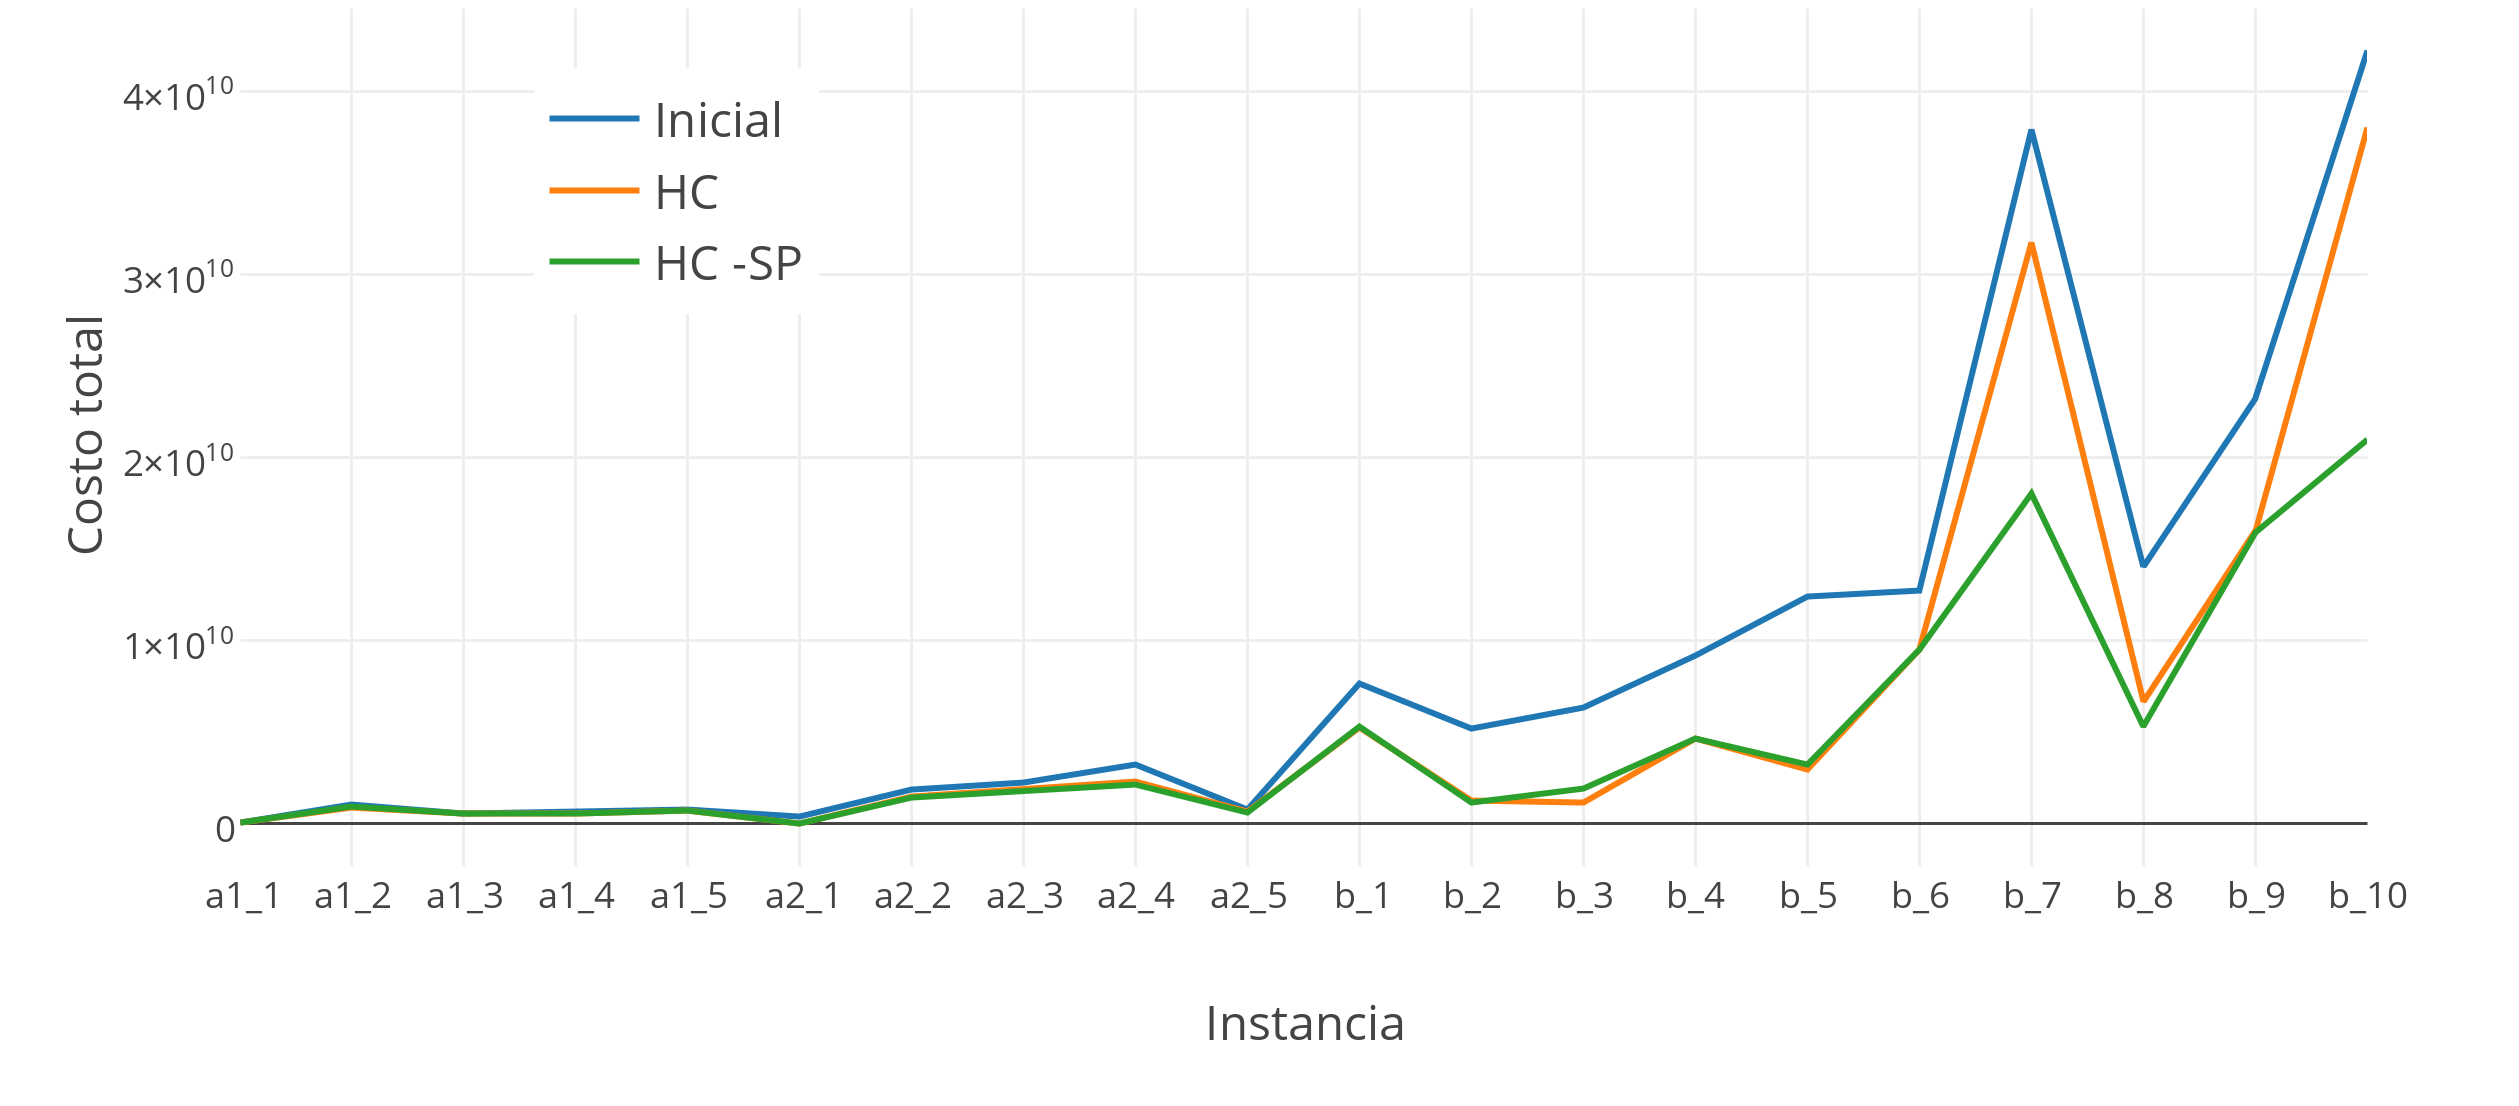
\includegraphics[width=0.45\textwidth]{comparativa-hc.png}
	\caption{\small}
	\label{fig:comparativa-hc}
\end{figure}

\begin{figure}[ht]
	\centering
	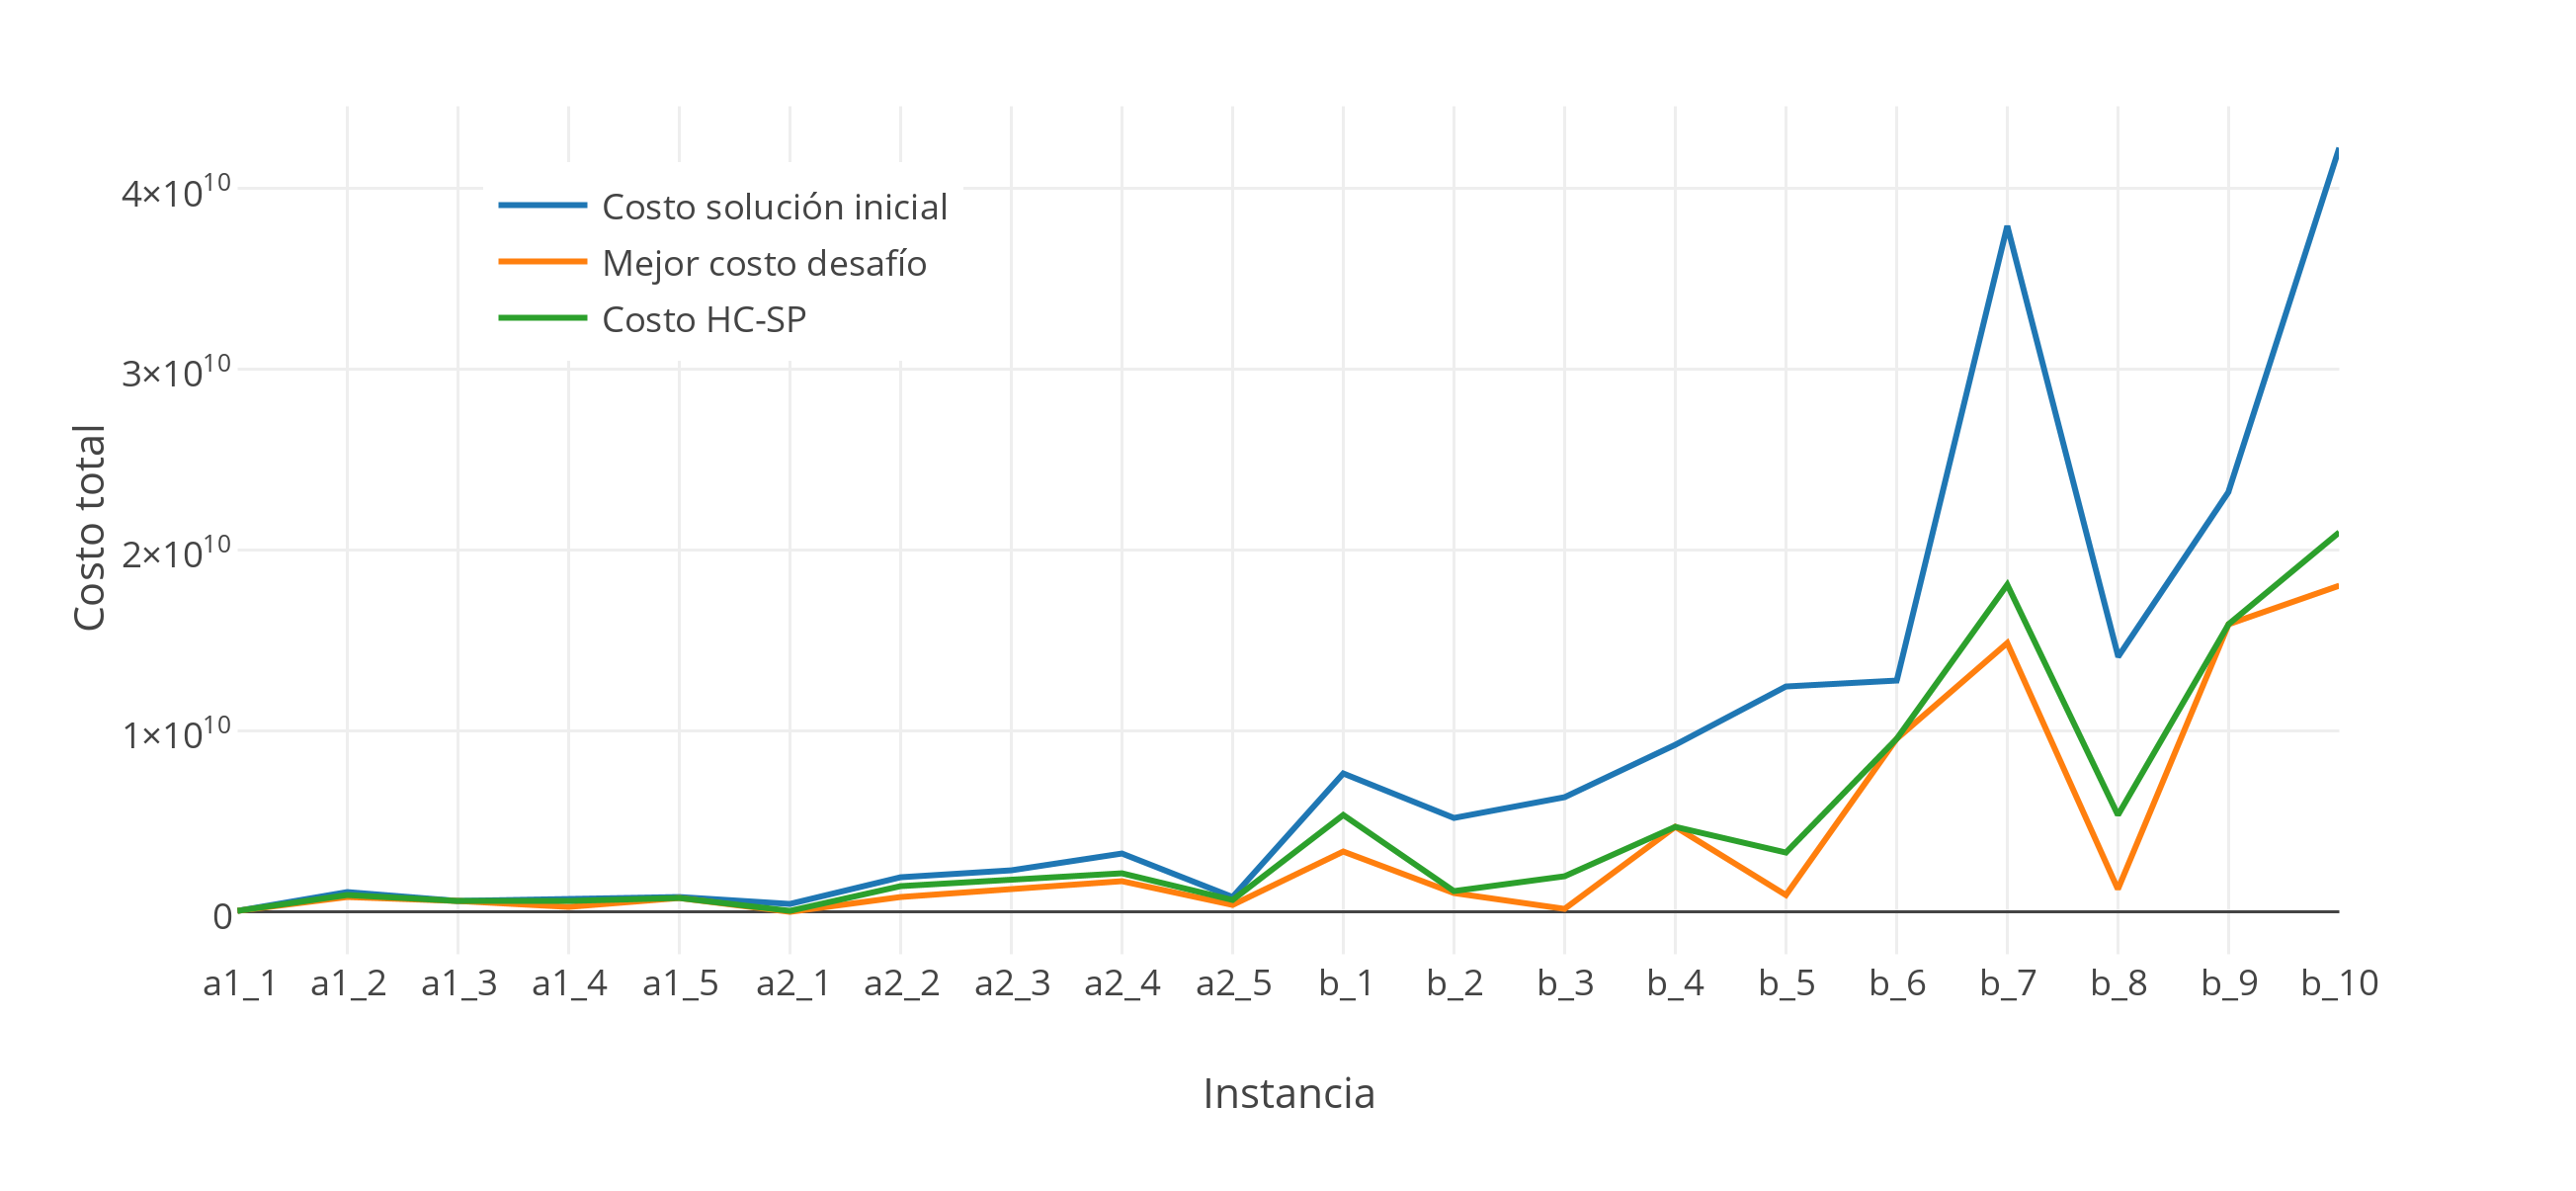
\includegraphics[width=0.45\textwidth]{comparativa-hc-best-challenge.png}
	\caption{\small}
	\label{fig:comparativa-hc-best-challenge}
\end{figure}


\end{document}


\section{Conclusiones}
\label{sec:conclusiones}
%Conclusiones RELEVANTES del estudio realizado. Debería responder a las preguntas: todas las técnicas resuelven el mismo problema o hay algunas diferencias?, En qué se parecen o difieren las técnicas en el contexto del problema?, qué limitaciones tienen?, qué técnicas o estrategias son las más prometedoras?, existe trabajo futuro por realizar?, qué ideas usted propone como lineamientos para continuar con investigaciones futuras?

En el presente informe se ha realizado una descripción en detalle del \mrp\, con una revisión de la literatura referente a las distintos algoritmos y técnicas desarrollados para la resolución del problema, considerando las metaheurísticas y representaciones utilizadas para aquello. \\
Cabe destacar que a pesar de lo novel del problema -publicado en la ROADEF/EURO 2012-, la naturaleza o estructura de éste no es algo nuevo en la investigación científica, puesto que el \mrp\ puede considerarse como una versión más restringida del \textit{Generalized Assignment Problem} o del \textit{Bin Packing Problem}. Sin embargo, dado el contexto actual en que los \textit{data centers} son piedras angulares en el funcionamiento de las organizaciones modernas y su gestión se vuelve una tarea sumamente crítica en la búsqueda de la efectividad y eficiencia, el \mrp\ por sí solo adquiere una relevancia importante. El hecho de que haya sido planteado por Google, corporación que basa la provisión de sus servicios a través del funcionamiento de extensas \textit{granjas} de servidores, es un indicativo de que para la industria de la ``nube'', los objetivos planteados por el  \mrp\ son críticos. \\
Respecto de las técnicas de resolución vistas en la sección \ref{sec:estado}, todas intentan solucionar el problema original publicado por Google. En general, dado que la presentación del problema se puede dar a través de instancias de gran tamaño, considerando por ejemplo 5000 máquinas, 50000 procesos y 12 recursos (descripción bastante cercana de la realidad que afrontan los gigantes informáticos), los algoritmos presentados utilizan esquemas de búsqueda local, que se aplican de forma iterativa sobre problemas de menor tamaño que el original, obtenidos a partir de un subconjunto de las máquinas y procesos involucrados, tratando de buscar asignaciones factibles y de bajo costo. A esto se suma que, el desafío original imponía un tiempo límite de ejecución para encontrar una solución de cinco minutos, por lo que los algoritmos en cuestión deben ser rápidos en la entrega de resultados, por lo que la utilización técnicas completas de búsqueda queda totalmente descartada. Esto se sustenta en el hecho de que los \textit{data centers} funcionan 24/7, por lo que el tiempo disponible para generar asignaciones que mejoren el uso de los servidores, es bastante limitado. Otro aspecto relevante y relacionado con el tamaño de las instancias del problema, es el de la representación. Como lo dejó establecido el trabajo de Mehta et al. \cite{mehta2012comparing}, la utilización de esquemas basados en \textit{Mixed Integer Programming} es bastante ineficiente para instancias de gran tamaño (con un espacio de búsqueda mayor, definición de una mayor cantidad de restricciones), por lo que la utilización del \textit{Constraint Programming} se es necesario para alcanzar una mayor escabilidad, especialmente cuando se utiliza una heurítica basada en LNS, combinación que entrega muy buenos resultados. Sin embargo, varios de los algoritmos vistos en el \textit{estado del arte} utilizan una representación basada en MIP (\cite{jaskowskihybrid}, \cite{lopes2015heuristics},\cite{masson2013iterated}), valiéndose del hecho de que dentro de ejecución iterativa, se resuelven subproblemas de menor tamaño. Estos problemas MIP, son resueltos luego mediante algún solver como CPLEX.\\
En relación al trabajo futuro, es destacable las mejoras que puede proveer la utilización de múltiples procesadores a la hora de ejecutar los distintos algoritmos. También sería importante pensar en la configuración automática y en tiempo real de los distintos parámetros de entrada que necesitan los algoritmos para ejecutarse, como por ejemplo la proporción de máquinas que se utilizarán para crear un subproblema.


% Conclusiones RELEVANTES del estudio realizado. Debería contener conclusiones del informe 1 junto con conclusiones obtenidas del desarrollo del software, análisis de resultados de experimentos y trabajo futuro.
  

 
\section{Bibliografía}
\bibliographystyle{plain}
\bibliography{informe2}
\end{document}